\documentclass[a4paper]{article}
\usepackage{vntex}
\usepackage{enumerate}
\usepackage{array}
\usepackage{enumitem}
\usepackage{hyperref}
\usepackage{graphicx}
\usepackage{caption}
\usepackage{pgfplots}
\usepackage{amssymb}
\usepackage{amsmath}
\usepackage{mathtools}
\usepackage{blkarray}
\usepackage{bookmark}
\usepackage{comment}
\usepackage[utf8]{inputenc}
\usepackage{anyfontsize}
\usepackage{pifont}
\usepackage{lastpage}
\usepackage{color}
\usepackage{natbib}
\usepackage{fancyhdr}
\usepackage{float}
\usepackage{tikz}
\usepackage[framemethod=tikz]{mdframed}
\usepackage{listings}
\usepackage{siunitx}
\usepackage{enumitem}
\usetikzlibrary{calc,backgrounds}
\newcommand\HRule{\rule{12cm}{1pt}}
\pagestyle{fancy}
\fancyhead{} % clear all header fields
\fancyhead[L]{
	\color{blue}
	\begin{tabular}{rl}
		\begin{picture}(25,15)(0,0)
		\put(0,-8){\includegraphics[width=8mm, height=8mm]{BK.png}}
		\end{picture}
		\begin{tabular}{l}
			\textbf{\bf \ttfamily Ho Chi Minh University of Technology}\\
			\textbf{\bf \ttfamily Faculty of Computer Science \& Engineering}
		\end{tabular} 	
	\end{tabular}
}
\fancyhead[R]{
	\begin{tabular}{l}
		\tiny \bf \\
		\tiny \bf 
	\end{tabular}
}
\fancyfoot{} % clear all footer fields
\fancyfoot[L]{\scriptsize \ttfamily Discrete Structures Assignment}
\fancyfoot[R]{\scriptsize \ttfamily Page {\thepage}/\pageref{LastPage}}
\renewcommand{\headrulewidth}{0.3pt}
\renewcommand{\footrulewidth}{0.3pt}

\begin{document}
	\begin{titlepage}
		\begin{tikzpicture}[remember picture, overlay]
		\draw[line width = 2pt] ($(current page.north west) + (1in,-1in)$) rectangle ($(current page.south east) + (-1in,1in)$);
		\end{tikzpicture}
		
		\begin{center}
			
			% Upper part of the page
			\textbf{\fontsize{12pt}{1pt}\selectfont HO CHI MINH CITY UNIVERSITY OF TECHNOLOGY}\\[0.5cm]
			{\fontsize{13pt}{1pt}\selectfont Faculty of Computer Science \& Engineering}\\[0.5cm]
			\begin{figure}[H]
				\centering
				\includegraphics[width=1.7in,height=1.7in]{BK.png}
			\end{figure}
			
			% Title
			\HRule \\[0.5cm]
			{ \textbf{\fontsize{25pt}{1pt}\selectfont Discrete Structures Assignment}}\\[0.4cm]
			
			\HRule \\[0.8cm]
			\begin{minipage}{0.545\textwidth}   
				\begin{flushleft} 
					\textbf{Authors:}\\
					\begin{tabular}{l l l}
						Nguyễn Hoàng & 1952255 & 25\% \\
						Tạ Minh Huy & 1952268 & 25\% \\
						Ho Trí Kháng & 1952069 & 25\% \\
						Nguyễn Khương & 1952310 & 25\% \\
					\end{tabular}
				\end{flushleft}
			\end{minipage}
			\begin{minipage}{0.4\textwidth}
				\begin{flushright} 
					\textbf{Class:}\\
					CO1007\\
					\textbf{Lecturer:}\\
					Trần Tuấn Anh\\
					
				\end{flushright}
			\end{minipage}
			
			\vfill
			
			% Bottom of the page
			\vspace{2cm}
			{\large} %{\large \today}
		\end{center}
	\end{titlepage}
	
	\pdfbookmark[0]{Counting}{counting}
	\section*{Counting}
	\pdfbookmark[1]{Problem 6}{cprob6}
	\subsection*{Problem 6:}
	A domino is a
	flat rectangular block, the face of which is divided into two square parts, each part showing from zero to six pips (or dots). Playing a game consists of playing dominoes with a matching number of pips. Explain why there are 28 dominoes in a complete set.\\\\
	\textit{Solution:}\\
	On a single dominoes, there are two parts, each of which can be assigned by a number from the set of ${0;1;2;3;4;5;6}$, this set has 7 elements.\\\\
	Therefore, exist ${7 \choose 2}$ combinations of 2 distinct number that can be put on dominoes.\\\\
	Also, there are dominoes which have the same number on both parts, with the set of 7 elements available. We got 7 distinct combinations of couples of the same number.\\\\
	Each combination form a different dominoes, then a complete set of dominoes should be the combined amount of both combination types, which is:
	\begin{equation*}
	   	21 + 7 = 28 \text{ (combinations / dominoes)}
	\end{equation*}

	\pdfbookmark[1]{Problem 7}{cprob7}
	\subsection*{Problem 7:}
	\begin{enumerate}
		\item How many solutions are there to the equation $x_1 + x_2 + x_3 + x_4 \leq 20$, where $x_1, x_2, x_3, x_4$ are non-negative integers? are positive integers?
		\item How many solutions are there to the equation $x_1 + x_2 + x_3 + x_4 = 20$, where $x_1, x_2, x_3, x_4$ are non-negative integers with $x_1 \leq 3, x_2 \geq 2, x_3 > 4$.
		\item How many ways to arrange 30 marbles in 5 different boxes, so that box 1 has at least 5 balls, knowing that box 2 and box 3 do not contain more than 6 balls.
	\end{enumerate}
	
	\textit{Solution:}
	\begin{enumerate}
		\item We can replace the equation with $x_1 + x_2 + x_3 + x_4 + x_5 = 20$ , where $x_1, x_2, x_3, x_4, x_5$ are non-negative integers. The number of solutions is 
		\begin{equation*}
		{n+r-1 \choose r}  = {24 \choose 20} = 10626
		\end{equation*}
		For $x_1, x_2, x_3, x_4$ are positive integers, decrease the RHS by 4, the problem becomes finding non-negative solutions to the equation: $x_1 + x_2 + x_3 + x_4 \leq 16$. The number of solutions is:
		\begin{equation*}
		{16+5-1 \choose 16} = 4845
		\end{equation*}
		\item Decrease the RHS by 7 (as $x_2 \geq 2, x_3 \geq 5$), the problem becomes finding non-negative solutions to the equation $x_1 + x_2 + x_3 + x_4 = 13$, such that $x_1 \leq 3$.\\
		Number of nonegative solutions to the above equation without constraint of $x_1$:
		\begin{equation*}
		    {13+4-1 \choose 13} = 560
		\end{equation*}
		    
		Number of solutions for $x_1 \geq 4$ can be calculated as:
		\begin{equation*}
            {9+4-1 \choose 9} = 220.
		\end{equation*}
		Using the rule of complement, number of solution where $x1 \leq 3$ equals the total number of solutions minus number of solutions where $x1 \geq 4$:
		\begin{equation*}
		560  - 220 = 340 \text{ (solutions).}		
		\end{equation*}
		\item We find non-negative solution to equation: $x_1 + x_2 + x_3 + x_4 + x_5 = 30$, where $x_1 \geq 5, x_2, x_3 \leq 6$.\\ 
		The problem can be rewritten as: $x_1 + x_2 + x_3 + x_4 + x_5 = 25$, where $ x_2, x_3 \leq 6$\\
		The number of solutions satisfying either $x_2$ or $x_3$ $\geq 7$ is: 
		\begin{equation*}
		{18+5-1 \choose 18} + {18 + 5 -1 \choose 18} - {11+5-1 \choose 11} = 13265.
		\end{equation*}
		Using the rule of compliment, the number of solutions where $x_2, x_3 \leq 6$ equals the total subtracted by n($x_2$ or $x_3 \geq 7$) :
		\begin{equation*}
		{25+5-1 \choose 25} - 13265 = 10486
		\end{equation*}
	\end{enumerate}
	
	
	\pdfbookmark[1]{Problem 8}{cprob8}
	\subsection*{Problem 8:}
	Given a set $A = \{1,2,3,4,5,6,7,8,9\}$.
	\begin{enumerate}
		\item From $A$ we can create how many sequence containing 5-different-digit numbers such that the middle number of this sequence is divisible by 5, number 5 appears only one, and the last number is an odd number?
		\item From $A$ we can create how many sequence containing 6-different-digit numbers such that the odd numbers cannot stand side by side (an odd number is not next to an odd number)?
		\item We can create how many odd numbers (a number includes 6-digit numbers from $A$) such that the number 5 always appears twice?
	\end{enumerate} 
	\textit{Solution:} \\
	\begin{enumerate}
	    \item The middle digit is 5, we have 8 digits left.\\
	    Choosing 1 of 4 odd digits for the last position, there are 4 ways. \\
	    Choosing 3 of 7 digits left to put on remaining 3 positions, there are $7\choose3$ ways. \\
	    There are:
	    \begin{equation*}
	        n = 4 \times {7 \choose 3} \times 3! =  840  \text{ (numbers). }
	    \end{equation*}
	    \item There are 2 cases satisfying :
	    \begin{itemize}
	        \item 4 evens, 2 odds :
	        \begin{equation*}
	           n_1 = 4! \times {5 \choose 2} \times {5 \choose 2} \times 2! = 4800 \text{ (numbers). }
 	        \end{equation*}
 	        \item 3 evens, 3 odds :
 	        \begin{equation*}
 	            n_2 = {4 \choose 3} \times 3! \times {4 \choose 3} \times {5 \choose 3} \times 3! = 5760 \text{ (numbers). }
 	        \end{equation*}
 	  
	    \end{itemize}
	    Totally, there are 10560 numbers satisfying.
	    \item There are 5 choices for the last digit that the number becomes odd: 1,3,5,7,9.
	    \begin{itemize}
	        \item Case 1: 5 is chosen \\
	        We need to choose 1 more position for 5 to appears, there are 5 ways. The remaining 4 positions, each has 8 possibilities (excluding number 5). 
	        There are:
	        \begin{equation*}
	            n_1 = 5 \times  8^{4} = 20480 \text{ (numbers). }
	        \end{equation*}
	        \item Case 2: 5 is not chosen \\
	        There are 4 possibilities for the last digit 1,3,7,9. \\
	        Pick up 2 of 5 remaining positions that 5 appears on: $ 5\choose 2$ ways.\\
	        The remaining 3 positions, each has 8 possibilities:
	        There are:
	        \begin{equation*}
	            n_2 = 4 \times {5 \choose 2} \times 8^{3} = 20480 \text{ (numbers). } 
	        \end{equation*}
	    \end{itemize}
	    Totally, there are 40960 numbers satisfying.
	\end{enumerate}
	\pdfbookmark[1]{Problem 9}{cprob9}
	\subsection*{Problem 9:}
	\begin{enumerate}
		\item Let $A$ be the set containing $n$ elements ($n > 4$). Assume there are $16n$ subsets of $A$ that have the number of elements is an odd number (the number of elements of each subset is an odd number). Find $n$?
		\item Let $A$ be the set containing $n$ elements ($n \geq 4$). Let $m$ be the number of subsets of $A$ which contains 4 elements, $k$ is the number of subsets of $A$ which contains 2 elements. Assume that $m = 20k$, find $n$?
	\end{enumerate}
	
	\textit{Solution:}
	\begin{enumerate}
		\item 
		The total subsets of a set n element is $2^n$.
		The number of odd subsets(subset has odd number of elements) and even subsets are both $2^{n-1}$
		\begin{align*}
		2^{n-1} &= 16n \\
		n &= 8
		\end{align*}
		\item m  = 20k\\
		Replacing m = ${n \choose 4}$ ,  $k = {n \choose 2}$:
		\begin{align*}
		&\frac{n!}{2\cdot(n-2)!} = \frac{n!}{24\cdot(n-4)!} \\
		&(n-4)\cdot(n-3) = 12 \\
		&n = 7
		\end{align*}
	\end{enumerate}
	
	\pdfbookmark[1]{Problem 10}{cprob10}
	\subsection*{Problem 10:}
	Given an equilateral triangle with the length of an edge is $n$. Separate this triangle into $n^2$ small equilateral triangles by using the parallel straight lines with the edges of the given triangle. Calculate the number of parallelograms located inside the given triangle.
	\begin{figure}[H]
		\centering
		\includegraphics[width=0.4\textwidth]{cprob10.png}
	\end{figure}
	
	\textit{Solution:}
	
	Given the equilateral triangle with edge length $n$, generate a parallelogram from the triangle with all edge lengths equal to $n$. Thus, we have two sets of parallel lines, each containing $n$ lines.
	
	We need to choose 2 lines from each set to create a parallelogram:
	\begin{equation*}
	{n \choose 2} \cdot {n \choose 2}
	\end{equation*}
	Because we are considering half of a parallelogram, we take half of the result above.
	\begin{align*}
	&\frac{1}{2} \cdot \frac{n!}{(n - 2)! \cdot 2!} \cdot \frac{n!}{(n - 2)! \cdot 2!} \\
	= &\frac{(n \cdot (n - 1))^2}{8} \\
	= &\frac{n^4 - 2 \cdot n^3 + n^2}{8} 
	\end{align*}
	
	\pdfbookmark[1]{Rosen's Book}{crosen}
	\subsection*{Rosen's Book}
	\pdfbookmark[2]{6.1.1}{c6.1.1}
	\subsubsection*{6.1.1:}There are 18 mathematics majors and 325 computer science majors at a college.
	\begin{enumerate}[label = \textbf{\alph*)}]
	    \item  In how many ways can two representatives be picked so that one is a mathematics major and the other is a computer science major?
	    \item In how many ways can one representative be picked who is either a mathematics major or a computer science major?

	\end{enumerate}
	\textit{Solution:}\\
	\begin{enumerate}[label = \textbf{\alph*)}]
	    \item Using rule of production. There are:
	    \begin{equation*}
	        18 \times 325 = 5850 \text{ (ways).}
	    \end{equation*}
	    \item Using rule of sum. There are:
	    \begin{equation*}
	        18 + 325 = 343 \text{ (ways).}
	    \end{equation*}
	\end{enumerate}
	\pdfbookmark[2]{6.1.20}{c6.1.20}
	\subsubsection*{6.1.20:}How many positive integers between 5 and 31
	\begin{enumerate}[label = \textbf{\alph*)}]
	    \item are divisible by 3? Which integers are these?
	    \item are divisible by 4? Which integers are these?
        \item are divisible by 3 and by 4? Which integers are these?
	\end{enumerate}
	\textit{Solution:} \\ 
	\begin{enumerate}[label = \textbf{\alph*)}]
	    \item 9 integers: 6,9,12,15,18,21,24,27,30.
	    \item 6 integers: 8,12,16,20,24,28.
        \item 2 integers: 12,24
	\end{enumerate}
	\pdfbookmark[2]{6.1.22}{c6.1.22}
	\subsubsection*{6.1.22:} How many positive integers less than 1000
	\begin{enumerate}[label = \textbf{\alph*)}]
	    \item are divisible by 7?
        \item are divisible by 7 but not by 11?
        \item are divisible by both 7 and 11?
        \item are divisible by either 7 or 11?
        \item are divisible by exactly one of 7 and 11?
        \item are divisible by neither 7 nor 11?
        \item have distinct digits?
        \item have distinct digits and are even?
	\end{enumerate}
	\textit{Solution:} \\
	Let A be the number of positive integers less than 1000. $A = 999$.
	\begin{enumerate}[label = \textbf{\alph*)}]
	    \item According to the quotient rule, number of integers which are divisible by 7 is:
	    \begin{equation*}
	        n_7 = \frac{A}{7} = \frac{999}{7} \approx 142.7143 \approx 142
	    \end{equation*}
        \item Number of integers divisible by 77:
	    \begin{equation*}
	        n_{77} = \frac{A}{77} = \frac{999}{77} = 12. 
	    \end{equation*}
	    Number of integers divisible by 7 but not 11:
	    \begin{equation*}
	        n_{7,not 11} = 142 - 12 = 130.
	    \end{equation*}
        \item Number of integers divisible by 77:
	    \begin{equation*}
	        \frac{A}{77} = \frac{999}{77} = 12. 
	    \end{equation*}
        \item Number of integers divisible by 11:
        \begin{equation*}
            n_{11} = \frac{999}{11} \approx 90.
        \end{equation*}
        According to the rule of intersection for 2 finite sets and the quotient rule, number of integers divisible by either 7 or 11 is:
	    \begin{equation*}
	        n_{7 or 11} = n_7 +n_{11} - n_{77} = 142 + 90 - 12 = 220. 
	    \end{equation*}
        \item The number of integers divisible by exactly 7 or 11 is the sum of numbers of integer divisible by 7 and 11, minus twice the number of integers divisible by 77:
        \begin{equation*}
            n = n_7 + n_{11} - 2n_{77} = 142 + 90 - 2\cdot 12 = 208.
        \end{equation*}
        \item Using the rule of complement, integers divisible by 7 nor 11 is the integers in the set that are not divisible by either 7 or 11:
        \begin{equation*}
            n_{not(7 or 11)} = A - n_{7 or 11} = 999 - 220 = 779
        \end{equation*}
        \item 
        \begin{itemize}
            \item 1 digit: 9 integers.
            \item 2 digits: 9 ways for the first digit(can not be 0) and 9 ways for the second digit(not the same as the first one).
            \item 3 digits: 9 ways for the first digit, 9 ways for the second digit(not the same as first one), 8 ways for the third digit(not the same as both first and second ones.)
        \end{itemize}
        Therefore, number of integers having distinct digits is where the number of digits less than or equal 3 is:
        \begin{equation*}
            9 + 9 \times 9 + 9 \times 9 \times 8 = 738.
        \end{equation*}

        \item  
        \begin{itemize} 
            \item 1 digit: 4 even integers.
            \item 2 digits: 
            \begin{itemize}
                \item[--] First digit: 9 ways.
                \item[--] Second digit: 5 if the first is odd and 4 if the first is even.
            \end{itemize}
            Totally, there are $5 \times 5 + 4\times 5 = 41$ 2-digit even integers.
            \item 3 digits: 9 ways(excluding '0') for the first digit and 9 ways for the second digit. For the third digit:
            \begin{itemize}
                \item[--] If first 2 digits are odd: 5 ways.
                \item[--] If first 2 digits are even: 3 ways.
                \item[--] If first is even and second is odd: 4 ways.
                \item[--] If first is odd and second is even: 4 ways.
            \end{itemize}
            Totally, number of 3-digit even integers is:
            \begin{equation*}
                5 \times 4 \times 5 + 4 \times 4 \times 3 + 4 \times 5 \times 4 + 5 \times 5 \times 4 = 328.
            \end{equation*}
        \end{itemize}
        All in all, there are $328 + 4 + 41 = 373$ ways.
	\end{enumerate}
        
	
	\pdfbookmark[2]{6.1.32}{c6.1.32}
	\subsubsection*{6.1.32:}How many strings of eight uppercase English letters are there
	\begin{enumerate}[label = \textbf{\alph*)}]
	    \item if letters can be repeated?
	    \item if no letter can be repeated?
        \item that start with X, if letters can be repeated?
        \item that start with X, if no letter can be repeated?
        \item that start and end with X, if letters can be repeated?
        \item that start with the letters BO (in that order), if letters can be repeated?
        \item that start and end with the letters BO (in that order), if letters can be repeated?
        \item that start or end with the letters BO (in that order), if letters can be repeated?
	\end{enumerate}
	\emph{Solution:}
	\begin{enumerate}[label = \textbf{\alph*)}]
	    \item Each letter has 26 possibilities from 'A' to 'Z'
	    \begin{equation*}
	        n = 26^{8} = 208827064576.
	    \end{equation*}
	    \item Since the letters have to be different:
	    \begin{equation*}
	        n = P(26,8) = 62990928000 
	    \end{equation*}
        \item There is only one way for the first letter(X) The remaining 7 letters, each has 26 possibilities: 
        \begin{equation*}
            n = 26^{7} = 8031810176
        \end{equation*}
        \item There is only one way for the first letter(X). The remaining 7 letters are not the same to each other, thus:
        \begin{equation*}
            n = 1 \times P(25,7) = 2422728000
        \end{equation*} 
        \item There is one way for the first and last letters(start and end with X). The remaining 6 letters, each has 26 possibilities:
        \begin{equation*}
            1 \times 26^{6} = 308915776
        \end{equation*}
        \item There is one way for the first two letters (BO). The remaining 6 letters, each has 26 possibilities:
        \begin{equation*}
            1 \times 26^{6} = 308915776
        \end{equation*}
        \item There is one way for the first and last two letters (BO and BO). The remaining 4 letters, each has 26 possibilities:
        \begin{equation*}
            1 \times 26^{4}
        \end{equation*}
        \item Using the subtraction rule and results of questions (f) and (g)
        \begin{equation*}
            n = n_{\text{start with }BO} + n_{\text{end with }BO} - n_{\text{start and end with }BO } = 26^{6} + 26^{6} - 26^{4} 
            = 617374576
        \end{equation*}
	\end{enumerate}
	\pdfbookmark[2]{6.1.50}{c6.1.50}
	\subsubsection*{6.1.50:} How many bit strings of length 10 contain either five consecutive 0s or five consecutive 1s?\\
	\textit{Solution:} \\
	There are 2 strings of length 10 contain both 5 consecutive 0s and 5 consecutive 1s: $1111100000$ and $0000011111$.\\
    To count the bit strings of length 10 containing at least 5 consecutive 0s, lets denote $k$ = the position that the first 0 of the sequence appears. As length is 10, $k \in \{1,2,3,4,5,6\}$ \\
    For $k = 1$, we have $2^{5}$ strings. (00000xxxxx) \\
    For $k > 1$, the $(k-1)^{th}$ bit must be 1, thus we have $2^{4}$ strings. (for example $k=2$ : 100000xxxx) \\
    Totally, the number of strings containing 5 consecutive 0s is : 
    \begin{equation*}
        2^{5} + 5\times 2^{4} = 112.
    \end{equation*}
    Similarly, number of strings containing 5 consecutive 1s is 112.\\
	By Inclusion-Exclusion, the result is:
	\begin{equation*}
	    n_{1 \text{ or } 0} = 112 + 112 - 2 = 222 \text{ (strings).}
	\end{equation*}
	\pdfbookmark[2]{6.1.51}{c6.1.51}
	\subsubsection*{6.1.51:}How many bit strings of length eight contain either three consecutive 0s or four consecutive 1s?\\
	\textit{Solution:} \\
	Let's A be the number of strings containing 3 consecutive 0s and B is the number of strings containing 4 consecutive 1s.
	\begin{enumerate} 
	    \item Three consecutive 0s can start from either 6 positions from $1^{th}$ to $6^{th}$.
	    \begin{itemize} 
	        \item[--] Case 1: start with 1st position 000xxxxx, any x can be chosen 2 ways hence total $2^5=32$ ways.
	        \item[--] Case 2: start with position 2,3 or 4, the position right before the first 0 is 1, there are $2^{4} $ ways. \\
	        For example, start at $3^{rd}$: x1000xxx, start at $4^{th}$: xx1000xx.
	        \item[--] Case 3: start with $5^{th}$ position, xxxx000x, $4^{th}$ x will be 1, position from 1 to 3 can be anything except 3 0s as 0001000x has already been counted in first case, there are 7 ways we can choose first three bits, and 2 ways to choose last 1 bit, total ways = 7*2 = 14 ways.
	        \item[--] Case 4: start at $6^{th}$, xxxxx000, $5^{th}$ position will be 1. First 4 bits can be chosen $2^4$ ways except 0000-1-000, 0001-1-000, 1000-1-000, hence there are only such 13 ways.
	    \end{itemize}
	    Totally, there are : $A= 32 + 3\times 2^{4} + 14+ 13 = 107$ ways.
	    \item Four consecutive 1's can start at either $1^{st},2^{nd},3^{rd}$ or $4^{th}$ position.
	    \begin{itemize}
	        \item[--] Case 1: start at $1^{st}$, 1111xxxx, there are $2^4 = 16$ ways.
	        \item[--] Case 2: start with position 2,3 or 4, the position right before the first 1 is 0, there are $2^{3} $ ways. (eg start at second position: 01xxxxxx )
	    \end{itemize}
	    Totally, there are : $B = 16 + 3\times 2^{3} = 48 $ ways.
	    \item For cases that contain both 3 consecutive 0s and 4 consecutive 1s, $|A \cap B| = 8$, as there are 2 possibilities for which streak comes first, 2 places to but the extra bit(either end), and 2 possibiities to put the extra bit's value.
	\end{enumerate}
	All in all, use the inclusive-exclusive principle to calculate number of strings that either contain 3 consecutive 0's or 4 consecutive 1's:
	\begin{equation*}
	    |A \cup B| = |A| + |B| - |A \cap B| = 107 + 48 - 8 = 147 \text{ (strings).}
	\end{equation*}
	\pdfbookmark[2]{6.2.1}{c6.2.1}
	\subsubsection*{6.2.1:}
	Show that in any set of six classes, each meeting regularly once a week on a particular day of the week, there must be two that meet on the same day, assuming that no classes are held on weekends.\\
	\textit{Solution:}\\
	By the pigeonholes: \\
	holes = day of the week except weekend = 5 = k \\
	objects = classes = 6 = k + 1 \\
	Each class only meets one day a week. Therefore, there must be at least 2 classes meet on the same day.
	\pdfbookmark[2]{6.2.10}{c6.2.10}
	\subsubsection*{6.2.10:}
	Let(xi, yi),i = 1, 2, 3, 4, 5, be a set of five distinct points with integer coordinates in the xy plane. Show that the midpoint of the line joining at least one pair of these points has integer coordinates.\\\\
	\textit{Solution:}\\
	To form a pair of integers as each point's coordinates, since an integer is either odd or even, there are only 4 possible combinations of parity possible:
	\begin{center}
	    ( odd ; odd )\\
	    ( odd ; even )\\
	    ( even ; odd )\\
	    ( even ; even )\\
	\end{center}
	There are 5 points but only 4 combinations of parity possible, according to the pigeonhole principle, there should be at least 2 points sharing the same combination of parity. We denoted them $A(x_i;y_i)$ and $B(x_j;y_j)$.\\\\
	Coordinates of the midpoint of these 2 points is ($\frac{x_i+x_j}{2}$;$\frac{y_i+y_j}{2}$).\\\\
	As these points share the same combinations of parity, $x_i$ and $x_j$ must be odd together or even together. It's impossible to get 1 odd - 1 even. Therefore, ($x_i + x_j$) must always be an even integer, and as a result, $\frac{x_i+x_j}{2}$ must always be an integer.\\\\
	At the same time, $y_i$ and $y_j$ must be odd together or even together. It's impossible to get 1 odd - 1 even. Therefore, ($y_i + y_j$) must always be an even integer, and as a result, $\frac{y_i+y_j}{2}$ must also always be an integer.\\\\
	In conclusion, there are always at least 1 pair of points whose midpoint has integer coordinates.
	\pdfbookmark[2]{6.2.17}{c6.2.17}
	\subsubsection*{6.2.17:}
	A company stores products in a warehouse. Storage bins in this warehouse are specified by their aisle, location in the aisle, and shelf. There are 50 aisles, 85 horizontal locations in each aisle, and 5 shelves throughout the ware-house. What is the least number of products the company can have so that at least two products must be stored in the same bin?\\
	\textit{Solution:}\\
	50 aisles, 85 horizontal locations in each aisle, and 5 shelves would have $50\times85\times5 = 21250$ bins.\\\\
	According to pigeonhole principle, with N holes there must be at least N+1 objects in order to have at least 1 hole contains more than one objects.\\\\
	Therefore, the least number of products the company can have so that at least two products must be stored in the same bin is 21250 + 1 = 21251.
	\pdfbookmark[2]{6.2.22}{c6.2.22}
	\subsubsection*{6.2.22:}
	Show that if there are 101 people of different heights standing in a line, it is possible to find 11 people in the order they are standing in the line with heights that are either increasing or decreasing.\\
	
	\textit{Solution: }\\ 
	Note that $101 = 10^2 + 1$. By Ramsey theory, every sequence containing $n^2 + 1$ distinct real numbers contains a subsequence of length $n+1$ that is either strictly increasing or decreasing. Apply with $n=10$, and it is proved that it is possible to find 11 people among those 101 people whose heights are either increasing or decreasing.
	
	\pdfbookmark[2]{6.2.38}{c6.2.38}
	\subsubsection*{6.2.38:}
	Find the least number of cables required to connect eight computers to four printers to guarantee that for every choice of four of the eight computers, these four computers can directly access four different printers. Justify your answer.\\
	
	\emph{Solution: }\\
	Connecting four computers to four printers requires $4\cdot 4=16$ cables. Now there is one group of four computers that has no access to the printers. Take one of them and connect to all the printers, which will require $4\cdot1=4$ cables. Thus, $16+4=20$ cables are needed.
	
	\pdfbookmark[2]{6.3.12}{c6.3.12}
	\subsubsection*{6.3.12:}
	\textit{Question:} How many bit strings of length 12 contain:
	\begin{enumerate} [label = (\alph*)]
		\item exactly three 1s? 
		\item at most three 1s?
		\item at least three 1s?
		\item an equal number of 0s and 1s?
	\end{enumerate}
	\textit{Solution:}\\
	\begin{enumerate} [label = (\alph*)]
		\item 
		\begin{align*}
		n_1 &= {12 \choose 3} = 220 \text{(strings)}
		\end{align*}
		\item 
		\begin{align*}
		n_2 &= {12 \choose 3} + {12\choose 2} + {12 \choose 1} + 1 = 299 \text{(strings)}
		\end{align*}
		\item 
		\begin{align*}
		n_3 &= 2^{12} - n_2 + n_1 = 4017 \text{(strings)}
		\end{align*}
		\item 
		\begin{align*}
		n_4 &= {12 \choose 6} = 924 \text{(strings)}
		\end{align*}
	\end{enumerate}
	
	\pdfbookmark[2]{6.3.18}{c6.3.18}
	\subsubsection*{6.3.18:}
	\textit{Question:} A coin is flipped eight times where each flip comes up
	either heads or tails. How many possible outcomes:
	\begin{enumerate} [label = (\alph*)]
		\item are there in total?
		\item contain exactly three heads?
		\item contain at least three heads?
		\item contain the same number of heads and tails?
	\end{enumerate}
	\textit{Solution:}\\
	\begin{enumerate} [label = (\alph*)]
		\item 
		\begin{align*}
		n &= 2^{8} = 256 \text{(outcomes)}
		\end{align*}
		\item 
		\begin{align*}
		n &= {8 \choose 3} = 56 \text{(outcomes)}
		\end{align*}
		\item 
		\begin{align*}
		n &= 256 - ( {8\choose 2} + {8 \choose 1} + 1) = 219 \text{(outcomes)}
		\end{align*}
		\item 
		\begin{align*}
		n &= {8 \choose 4} = 70 \text{(outcomes)}
		\end{align*}
	\end{enumerate}
	
	\pdfbookmark[2]{6.3.21}{c6.3.21}
	\subsubsection*{6.3.21:}
	\textit{Question:} How many permutations of the letters ABCDEFG contain
	\begin{enumerate} [label = (\alph*)]
		\item the string BCD?
		\item the string CFGA?
		\item the strings BA and GF?
		\item the strings ABC and DE?
		\item the strings ABC and CDE?
		\item the strings CBA and BED?
	\end{enumerate}
	\textit{Solution:} 
	\begin{enumerate} [label = (\alph*)]
		\item We treat the given string as one singular letter. In this case, we have 5 possible letters: A, BCD,E,F,G. The number of permutations is: 
		\begin{align*}
		n &= 5! = 120 \text{(permutations)}
		\end{align*}
		\item Similar to question (a), there are 4 possible letters :
		\begin{align*}
		n &= 4! = 24 \text{(permutations)}
		\end{align*}
		\item We treat two given strings as two singular letters. There are 5 possible letters: BA,C,D,E,GF
		\begin{align*}
		n &= 5! = 120 \text{(permutations)}
		\end{align*}
		\item Similar to question (c):
		\begin{align*}
		n &= 4! = 24 \text{(permutations)}
		\end{align*}
		\item Since the new string contain ABC and CDE, the string must contain ABCDE. There are 3 possible letters : ABCDE,F,G:
		\begin{align*}
		n &= 3! = 6 \text{(permutations)}
		\end{align*}
		\item There is no way that a string contain both CBA and BED, thus:
		\begin{align*}
		n &= 0 \text{(permutations)}
		\end{align*}
	\end{enumerate}
	\pdfbookmark[2]{6.3.25}{c6.3.25}
	\subsubsection*{6.3.25:}
	One hundred tickets, numbered 1, 2, 3, ..., 100, are sold to 100 different people for a drawing. Four different prizes are awarded, including a grand prize (a trip to Tahiti). How many ways are there to award the prizes if
	\begin{enumerate}[label = \textbf{\alph*)}]
		\item there are no restrictions?
		\begin{align*}
		P(100,4) & = \frac{100!}{(100-4)!} \\
		& = 94109400
		\end{align*}
		\item the person holding ticket 47 wins the grand prize? \\
		Person holding ticket 47 wins the grand prize, so we need to pick the remaining 3 prizes.
		\begin{align*}
		P(100,4) & = \frac{99!}{(99-3)!} \\
		& = 941094
		\end{align*}
		\item the person holding ticket 47 wins one of the prizes? \\
		There are 4 prizes for the person to win, so we need to pick the remaining 3 people. From part (b), we have the number of ways to pick 3 prizes.
		\begin{equation*}
		4 \cdot 941094 = 3764376
		\end{equation*}
		\item the person holding ticket 47 does not win a prize?
		\begin{align*}
		P(99,4) & = \frac{99!}{(99-4)!} \\
		& = 90345024
		\end{align*}
		\item the people holding tickets 19 and 47 both win prizes. \\
		First, we need to distribute 2 prizes amongst 4 people.
		\begin{align*}
		P(4,2) & = \frac{4!}{(4-2)!} \\
		& = 12
		\end{align*}
		Then, we need to select 2 prizes for the remaining 98 people.
		\begin{align*}
		P(98,2) & = \frac{98!}{(98-2)!} \\
		& = 9506
		\end{align*}
		By the product rule
		\begin{equation*}
		12 \cdot 9506 = 114072
		\end{equation*}
		\item the people holding tickets 19, 47, and 73 all win prizes? \\
		First, we need to distribute 3 prizes amongst 4 people.
		\begin{align*}
		P(4,3) & = \frac{4!}{(4-3)!} \\
		& = 24 
		\end{align*}
		Then, we need to select 1 prize for the remaining 97 people.
		\begin{align*}
		P(97,1) & = \frac{97!}{(97-1)!} \\
		& = 97
		\end{align*}
		By the product rule
		\begin{equation*}
		24 \cdot 97 = 2328
		\end{equation*}
		\item the people holding tickets 19, 47, 73, and 97 all win prizes? \\
		We need to choose 4 prizes for 4 people.
		\begin{align*}
		P(4,4) & = \frac{4!}{(4-4)!} \\
		& = 24
		\end{align*}
		\item none of the people holding tickets 19, 47, 73 and 97 wins a prize? \\
		We need to choose 4 prizes for the remaining 96 people.
		\begin{align*}
		P(96,4) & = \frac{96!}{(96-4)!} \\
		& = 79727040
		\end{align*}
		\item the grand prize winner is a person holding ticket 19, 47, 74, or 97? \\
		First, we need to pick 1 person from 4 people to reward a grand prize.
		\begin{align*}
		P(4,1) & = \frac{4!}{(4-1)!} \\
		& = 4
		\end{align*}
		Then, we need to select 3 prizes for the remaining 99 people.
		\begin{align*}
		P(99,3) & = \frac{99!}{(99-3)!} \\
		& = 941094
		\end{align*}
		By the product rule
		\begin{equation*}
		4 \cdot 941094 = 3764376	
		\end{equation*}
		\item the people holding tickets 19 and 47 win prizes, but the people holding tickets 73 and 97 do not win prizes? \\
		First, we need to distribute 2 prizes amongst 4 people.
		\begin{align*}
		P(4,2) & = \frac{4!}{(4-2)!} \\
		& = 12
		\end{align*}
		Then, we need to select 2 prizes for the remaining 96 people.
		\begin{align*}
		P(96,2) & = \frac{96!}{(96-2)!} \\
		& = 9120
		\end{align*}
		By the product rule
		\begin{equation*}
		12 \cdot 9120 = 109440
		\end{equation*}
	\end{enumerate}
	
	\pdfbookmark[2]{6.3.38}{c6.3.38}
	\subsubsection*{6.3.38:}
	How many ways are there to select 12 countries in the United Nations to serve on a council if 3 are selected from a block of 45, 4 are selected from a block of 57, and the others are selected from the remaining 69 countries?
	\begin{align*}
	n &=  {45 \choose 3}{57 \choose 4}{69 \choose 5} \\
	&=  62994022035644700 \text{ (ways).}
	\end{align*}
	
	\pdfbookmark[2]{6.4.9}{c6.4.9}
	\subsubsection*{6.4.9:}
	What is the coefficient of $x^{101}y^{99}$ in the expansion of $(2x - 3y)^{200} ?$\\
	\emph{Solution:}
	\begin{equation*}
	   (2x - 3y)^{200} = \sum_{k=0}^{200} {200 \choose k}(2x)^{200-k}(-3y)^{k} = \sum_{k=0}^{200} {200 \choose k} 2^{200-k}(-3)^{k} x^{200 -k}y^{k}
	\end{equation*}
	$x^{101}y^{99}$ corresponds to $k=99$. The coefficient is : $-{200 \choose 99}2^{101}3^{99}$
	\pdfbookmark[2]{6.4.10}{c6.4.10}
	\subsubsection*{6.4.10:}
	Give a formula for the coefficient of $x^{k}$ in the expansion of $(x + 1/x)^{100}$, where k is an integer. \\
	\emph{Solution:}
	\begin{equation*}
	    (x + \frac{1}{x})^{100} = \sum_{l = 0}^{100} {100 \choose l} x^{100 - 2l}
	\end{equation*}
	$x^{k}$ corresponds to $l = \frac{100-k}{2}$. So the coefficient of $x^{k}$ is :
	\begin{equation*}
	    x^{k} = {100 \choose {\frac{100-k}{2}}} = \frac{100!}{(\frac{100-k}{2})!(\frac{100+k}{2})!}
	\end{equation*}
	\pdfbookmark[2]{6.4.15}{c6.4.15}
	\subsubsection*{6.4.15:}
	Show that ${n \choose k} \leq 2^n$ for all positive integers $n$ and all integers $k$ with $0 \leq k \leq n$.\\
	\textit{Solution:}\\
	Suppose we have integers $n$ and $k$ satisfying $0 \leq k \leq n$
	\begin{align*}
	2^n & = (1+1)^n \\
	& = \sum_{i=0}^{n} {n \choose i} 1^{n-i}\;1^i \\
	& = \sum_{i=0}^{n} {n \choose i} \geq {n \choose k}
	\end{align*}
	
	\pdfbookmark[2]{6.4.20}{c6.4.20}
	\subsubsection*{6.4.20:}
	Suppose that $k$ and $n$ are integers with $1 \leq k \leq n$. Prove the \textbf{hexagon identity}
	\begin{equation*}
	    {n-1 \choose k-1}{n \choose k+1}{n+1 \choose k} = {n-1 \choose k}{n \choose k-1}{n+1 \choose k+1}
	\end{equation*}
	which relates terms in Pascal's triangle that form a hexagon. \\
	\textit{Solution:} \\
	\begin{align*}
	& {n-1 \choose k-1}{n \choose k+1}{n+1 \choose k} \\
	= & \frac{(n-1)!}{(k-1)!(n-k)!} \frac{n!}{(k+1)!(n-k-1)!} \frac{(n+1)!}{k!(n+1-k)!} \\
	= & \frac{(n-1)!}{k!((n-1)-k)!} \frac{n!}{(k-1)!(n-(k-1))!} \frac{(n+1)!}{(k+1)(n-k)!} \\
	= & \frac{(n-1)!}{k!((n-1)-k)!} \frac{n!}{(k-1)!(n-(k-1))!} \frac{(n+1)!}{(k+1)((n+1)-(k+1))!} \\
	= & {n-1 \choose k}{n \choose k-1}{n+1 \choose k+1}
	\end{align*}
	
	\pdfbookmark[2]{6.4.25}{c6.4.25}
	\subsubsection*{6.4.25:} Let $n$ be a positive integer. Show that: 
	\begin{equation*}
	    {{2n} \choose {n+1}} + {{2n} \choose {n}} = \frac{{{2n+2} \choose {n+1}}}{2}
	\end{equation*}
	\textit{Solution:} \\
	Using Pascal Identity :
	\begin{align*}
	   {{2n} \choose {n+1}} + {{2n} \choose {n}} &= {{2n+1} \choose {n+1}} \\
	   &= \frac{(2n+1)!}{(n+1)!(n)!} \\
	   &= \frac{(2n+1)!}{(n+1)!(n)!} \cdot \frac{2n+2}{2n+2} \\
	   &= \frac{(2n+2)!}{2(n+1)!(n+1)!} \\
	   &= \frac{(2n+2)!}{2(n+1)!((2n+2)-(n+1))!} \\
	   &= \frac{{{2n+2} \choose {n+1}}}{2} \text{ (Q.E.D)} \\
	\end{align*} 
	
	\pdfbookmark[2]{6.4.60}{c6.4.60}
	\subsubsection*{6.4.30:}
	Give a combinatorial proof that:
	\begin{equation*}
	    \sum_{k=1}^{n} k{n \choose k}^{2} = n{{2n-1}\choose{n-1}}
	\end{equation*}
	[ Hint:Count in two ways the number of ways to select a committee, with $n$ members from a group of $n$ mathematics professors and $n$ computer science professors, such that the chairperson of the committee is a mathematics professor. ]\\
	\textit{Solution:} \\
	\begin{enumerate}
	    \item Choose k members from mathematics in ${n \choose k}$ ways and (n-k) remaining members from computer science in ${n\choose{n-k}} = {n \choose k}$ ways, where $k \geq 1$ as we need to choose at least one from mathematics to have a chair person from there. Then the chairperson can be chosen from selected members of mathematics in k ways.
	    \item First choose the chairperson from mathematics in $n$ ways and then the remaining $n-1$ members can be selected from the rest of the $(2n -1)$ combined population in ${{2n-1}\choose{n-1}}$ ways.
	\end{enumerate}
	\newpage
	\pdfbookmark[0]{Probability}{probability}
	\section*{Probability}
	\pdfbookmark[1]{Problem 1}{pprob1}
	\subsection*{Problem 1:}
	Suppose that 8\% of the patients tested in a clinic are infected with HIV. Furthermore, suppose that when a blood test for HIV is given, 98\% of the patients infected with HIV test positive and that 3\% of the patients not infected with HIV test positive. What is the probability that infected with it? \\
	
	Let	I be patient infected with HIV and T be patient tested positive with HIV.
	\begin{align*}
	p(I) &= 0.08 \\
	p(T|I) &= 0.98 \\
	p(T|\overline{I}) &= 0.03
	\end{align*}
	\begin{enumerate}
		\item a patient testing positive for HIV with this test is infected with it?
		\begin{align*}
		p(I|T) &= \frac{p(T|I) \cdot p(I)}{p(T|I) \cdot p(I) + p(T|\overline{I}) \cdot p(\overline{I})} \\
		&= \frac{0.98 \cdot 0.08}{0.98 \cdot 0.08 + 0.03 \cdot 0.92} \\
		&= 0.74
		\end{align*}
		\item a patient testing positive for HIV with this test is not infected with it?
		\begin{align*}
		p(\overline{I}|T) &= \frac{p(T|\overline{I}) \cdot p(\overline{I})}{p(T|\overline{I}) \cdot p(\overline{I}) + p(T|I) \cdot p(I)} \\
		&= \frac{0.03 \cdot 0.92}{0.03 \cdot 0.92 + 0.98 \cdot 0.08} \\
		&= 0.26
		\end{align*}
		\item a patient testing negative for HIV with this test is infected with it?
		\begin{align*}
		p(I|\overline{T}) &= \frac{p(\overline{T}|I) \cdot p(I)}{p(\overline{T}|I) \cdot p(I) + p(\overline{T}|\overline{I}) \cdot p(\overline{I})} \\
		&= \frac{0.02 \cdot 0.08}{0.02 \cdot 0.08 + 0.97 \cdot 0.92} \\
		&= 0.0018
		\end{align*}
		\item a patient testing negative for HIV with this test is not?
		\begin{align*}
		p(\overline{I}|\overline{T}) &= \frac{p(\overline{T}|\overline{I}) \cdot p(\overline{I})}{p(\overline{T}|\overline{I}) \cdot p(\overline{I}) + p(\overline{T}|I) \cdot p(I)} \\
		&= \frac{0.97 \cdot 0.92}{0.97 \cdot 0.92 + 0.02 \cdot 0.08} \\
		&= 0.998
		\end{align*}
	\end{enumerate}
	
	\pdfbookmark[1]{Problem 2}{pprob2}
	\subsection*{Problem 2:}
	The final exam of a discrete mathematics course consists of 50 true/false questions, each worth two points, and 25 multiple-choice questions, each worth four points. The probability that Linda answers a true/false question correctly is 0.9, and the probability that she answers a multiple-choice question correctly is 0.8. What is her expected score on the final? \\
	\textit{Solution:} \\
	\begin{math}
	E(true/false) = n_{true/false} \cdot P_{true/false} = 50 \cdot 0.9 = 45 \\
	E(multiple) = n_{multiple} \cdot P_{multiple} = 25 \cdot 0.8 = 20
	\end{math} \\
	Total expected point: $2\cdot45+4\cdot20=170$.
	
	\pdfbookmark[1]{Problem 3}{pprob3}
	\subsection*{Problem 3:}
	Please consider the poker rule via this link: $\href{https://en.wikipedia.org/wiki/List_of_poker_hands}{https://en.wikipedia.org/wiki/List\_of\_poker\_hands}$. Following this rule, what is the probability that a poker hand contains: Straight flush, Four of a kind, Full house, Flush, Straight, Three of a kind, Two pair, One pair, High card? \\
	\textit{Solution:}\\
	Pick up randomly 5 from 52 cards, the sample space is :  ${52 \choose 5}$
	\begin{enumerate}
		\item Straight flush\\
		Choose one of four suits, there are 4 ways. \\
		Pick up 5 consecutive cards of that suit, there are 10 ways \\
		Totally, there are 10*4 = 40 ways
		\begin{align*}
		&p = \frac{40}{{52\choose 5}} \approx \num{1.54e-5} 
		\end{align*}
		\item Four of a kind \\
		There are 13 different ranks, choose one of them: 13 ways.
		Thus there are 13 ways to pick up 4 cards of the same rank. \\
		To pick up the remaining card, there are 48 ways.
		\begin{align*}
		p = \frac{13\times48}{{52\choose 5}} \approx \num{2.4e-4}
		\end{align*}
		\item Full house \\
		Choose one of 13 ranks: 13 ways \\
		Pick up 3 cards of that rank(there are 4 corresponding to 4 suits): ${4 \choose 3}$ ways. \\
		Choose one of 12 remaining ranks: 12 ways. \\
		Pick up 2 cards of that rank: ${4\choose 2}$ ways. \\
		\begin{align*}
		p = \frac{13 \times {4\choose 3} \times 12 \times {4 \choose 2}}{{52 \choose 5}} = \num{1.44e-3} 
		\end{align*}
		\item Flush \\
		Pick up 5 cards of the same suits, there are : $4 \times{13\choose 5}$ ways. \\
		Excluding cases where straight flush appears: 
		\begin{align*}
		p = \frac{4 \times {13 \choose 5} - 40}{{52 \choose 5}} \approx \num{1.97e-3}
		\end{align*}
		\item Straight \\
		Pick up 5 consecutive cards: 10 ways\\
		Each card in the sequence has 4 possibilities. Excluding the straight flush:\\
		\begin{align*}
		p = \frac{10 \times 4^{5} - 40 }{{52 \choose 5}} \approx \num{3.92e-3}
		\end{align*}
		\item Three of a kind \\
		Pick up 3 cards of the same rank : $13\times {4 \choose 3}$ ways. \\
		The remaining 2 cards neither make up a pair nor share the same rank as the first 3 ones: ${12\choose 2} \times 4^{2}$ ways.
		\begin{align*}
		p = \frac{13\times {4 \choose 3}\times{12 \choose 2}\times 4^{2} }{{52\choose 5}} \approx 0.0211
		\end{align*}
		\item Two pairs\\
		Pick up 2 pairs: ${13 \choose 2}\times {4 \choose 2}^{2}$ ways. \\
		The remaining card: 44 ways. \\
		\begin{align*}
		p = \frac{{13 \choose 2}\times {4 \choose 2}^{2} \times 44}{{52 \choose 5}} \approx 0.048
		\end{align*}
		\item One pair\\
		Pick up one pair: $13 \times {4 \choose 2}$ ways. \\
		The remaining 3 cards: ${12 \choose 3} \times {4 \choose 1}^{3}$ ways. \\
		\begin{align*}
		p = \frac{13 \times {4 \choose 2} \times {12 \choose 3} \times {4 \choose 1}^{3}}{{52 \choose 5}} \approx 0.42
		\end{align*}
		\item High card \\
		Pick up 5 cards of different ranks not making a straight: $({13 \choose 5}-10)\times 4^{5}$ ways. \\
		Exclude cases of flush : $({13 \choose 5}-10)\times 4$ cases. \\
		\begin{align*}
		p = \frac{({13 \choose 5}-10)\times (4^{5}-4)}{{52 \choose 5}} \approx 0.50
		\end{align*}
	\end{enumerate}
	\pdfbookmark[1]{Problem 4}{pprob4}
	\subsection*{Problem 4:}
	\begin{enumerate}
		\item A group containing 20 people (5 men and 15 women) is randomly assigned to 4 different groups (each group has 5 people). Calculate the probability that females will be in the same group? \\
		\textit{Solution:}\\
		To divide 20 people into 4 different group. We consecutively setting up each groups as
		\begin{equation*} 
		    {20 \choose 5} \times {15 \choose 5} \times {10 \choose 5} \times {5 \choose 5}
		\end{equation*}
		5 men will be in the same group. Pick up 1 out of 4 groups: 4 ways. \\
		Dividing 15 women in the remaining 3 groups: ${15 \choose 5} \times {10 \choose 5} \times {5 \choose 5}$ ways \\
		The probability is: 
		\begin{equation*}
		    p = \frac{4 \times {15 \choose 5} \times {10 \choose 5} \times {5 \choose 5}}{{20 \choose 5} \times {15 \choose 5} \times {10 \choose 5}}  = \frac{1}{3876} \approx \num{2.58e-4}
		\end{equation*}
		\item A phone number consisting of 9 random numbers, a man forgets two last digits of the phone number. However, he knows that the two digits are different. He chooses these two numbers randomly, find the probability that he calls the correct number?\\\\
		\textit{Solution:}
		Digits are chosen from a set from 0 to 9, which has 10 elements.\\\\
		Number of permutations of 2 different numbers (order is considered) is $A_{2}^{10}$ = 90.\\\\
		There is only 1 correct permutation. Then the probability is:
		\begin{equation*}
		    \frac{1}{90} \approx 0.0111 
		\end{equation*}
		
		
		\item Arrange 7 people consisting of four sons, two daughters, and a child sitting in seven chairs around a round-table. What is the probability of a child sitting between two girls?\\\\
		\textit{Solution:}
		For a round table, there is no first nor last seat as it was in rows of seat. Therefore, we only count considering the relations between people.\\\\
		First, the amount of all possible ways to get 7 persons into 7 seats is (7-1)!.Since we have to get 1 person to sit first as a marking point, then randomly settled the other 6 in 6 seats respected to the first one's seat, we got in total 6! = 720 possible ways\\\\
		Then, to match the condition, we're placing the two women on either side of the child. There are 2 ways for the two women to sit.\\\\
		The four men can sit wherever they'd like in the remaining seats, which is: 
		\begin{equation*}
		    4! = 24 \text{ (ways)}
		\end{equation*}
		All together then, we have: 
		\begin{equation*}
		    2 \times 24 = 48 \text{ (ways)}
		\end{equation*}
		The probability should be: 
		\begin{equation*}
		    \frac{48}{720} \approx 0.0667 
		\end{equation*}
		\item Roll three dice at the same time, knowing that at least one of them is five dots. Calculate the probability that the total number of dots of 3 dice is 8?\\\\
		\textit{Solution:} \\
		Rolling 3 dices with at least one is five dots, there are 3 cases of choosing dices to be 5 \\\\
		Since the chosen dice got the constant value of 5, it has only 1 value to take. For each of 2 other dices, there are 6 values available, therefore the number of all possible outcome is:
		\begin{equation*}
		    3\times1\times6\times6 = 108
		\end{equation*}
		To get the total value of 8 out of 3 dices, with one being 5. the only combinations possible is 
		\begin{equation*}
		    (5;1;2)
		\end{equation*}
		With each values assigned to the dices. Now it all comes down to counting ways of assigning 3 values to 3 dices, which is 3! = 6.\\\\
		The probability then become:
		\begin{equation*}
		    \frac{6}{108} = \frac{1}{18} \approx 0.0556 
		\end{equation*}
		\item A soccer tournament has 12 teams, 9 teams are foreign and 3 teams are domestic. The organizers want to divide 12 teams into 3 groups A, B, C (4 teams per group). Calculate the probability that three domestic teams are in three different tables.\\\\
		\textit{Solutions:} \\
		To set up 3 tables of 4 teams from 12 teams, there are in total
		\begin{equation*}
		{12\choose4}\times{8\choose4}\times{4\choose4} = 34650 \text{ (ways)}
		\end{equation*}
		For 3 domestic teams to be in different table, we settled them first. (order considered) The number of ways to put 3 teams in 3 different tables is
		\begin{equation*}
		    3! = 6
		\end{equation*}
		After that, we put the remaining 9 teams in 3 teams:
		\begin{equation*}
		{9\choose3}\times{6\choose3}\times{3\choose3} = 1680	\end{equation*}
		The probability is relatively: 
		\begin{equation*}
		    \frac{6\times1680}{34650} = \frac{16}{55} \approx 0.2901
		\end{equation*}
		\item Let A, B, C be any events. Prove that: \\
		\begin{math}
		P(A \cup B \cup C) = P(A) + P(B) + P(C) - P(A \cap B) - P(B \cap C) - P(A \cap C) + P(A \cap B \cap C)
		\end{math}\\
		\textit{Solutions:}\\
		\begin{math}
		P(A \cup B \cup C) \newline 
		= P(A \cup B) + P(C) - P((A \cup B)\cap C))
		\newline
		=P(A \cup B) + P(C) - P((A\cap C) \cup (B\cap C))
		\newline
		=P(A) +P(B) - P(A \cap B) + P(C) - ( P(A \cap C) + P(B \cap C) - P(A \cap B \cap C) )
		\newline
		=P(A) + P(B) + P(C) - P(A \cap B) - P(B \cap C) - P(A \cap C) + P(A \cap B \cap C)
		\end{math}
		\item Suppose that E and F are events such that $p(E) = 0.7$ and $p(F) = 0.5$. Show that $p(E \cup F) \geq 0.7$ and $p(E \cap F) \geq 0.2$\\
		\textit{Solution:}\\\\
		The union E $\cup$ F contains all outcomes of E and F.
		Therefore, the probability of the sum must be at least the probability of either E or F\\\\
		\begin{equation*}
		P(E\cup F) \geq P(F) = 0.5
		\end{equation*}
		\begin{equation*}
		P(E\cup F) \geq P(E) = 0.7
		\end{equation*}
		According to the above reasoning, we have 
		\begin{equation*}
		P(E\cup F) \geq 0.7
		\end{equation*}
		Also, all probabilities can't exceed 1 (100\%), therefore\\
		\begin{equation*}
		P(E\cup F) \leq 1
		\end{equation*}
		\begin{equation*}
		P(E) + P(F) - P(E \cap F) \leq 1
		\end{equation*}
		\begin{equation*}
		0.5 + 0.7 - P(E \cap F) \leq 1
		\end{equation*}
		\begin{equation*}
		P(E \cap F) \geq 1.2 - 1 
		\end{equation*}
		\begin{equation*}
		P(E \cap F) \geq 0.2
		\end{equation*}
		
	\end{enumerate}
	
	\pdfbookmark[1]{Problem 5}{pprob5}
	\subsection*{Problem 5:}
	To go to school, a student must cross a railroad track. The time trains run through this rail are a little bit different every day. However, this student estimates she has to wait for the train approximately 15\% of the school days. During one week of schooling there are 5 days, the probability will be how much if this student
	\begin{enumerate}
		\item Sees a train on Monday and do it again on Tuesday?
		\begin{equation*}
		0.15 \cdot 0.15 = 0.0225
		\end{equation*}
		\item The first time she meets a train is Thursday?
		\begin{equation*}
		0.85^3 \cdot 0.15 \approx 0.0921
		\end{equation*}
		\item Sees a train everyday?
		\begin{equation*}
		0.15^5 \approx \num{7.59e-5}
		\end{equation*}
		\item Sees a train at least once a week? \\
		Using the rule of compliment, the probability is: 
		\begin{equation*}
		1 - 0.85^5 \approx 0.5563
		\end{equation*}
	\end{enumerate}
	
	\pdfbookmark[1]{Problem 6}{pprob6}
	\subsection*{Problem 6:}
	A straight iron rod of length $l$ (unit length) is cut randomly into three pieces. Find the probability that these three iron pieces form a triangle. \\
	\textit{Solution: } \\
	Lets x,y be the first 2 pieces, the length of the remaining piece is (l -x -y).
	For the three pieces to form a triangle, the triangle inequality must be true:
	\begin{align*}
	    x + y > l- x -y  &=> x+y > \frac{l}{2} \\
	    x + l -x -y > y &=> y < \frac{l}{2} \\
	    y + l - x - y > x &=> x < \frac{l}{2} \\
	\end{align*}
	We can easily see that the area of the triangle formed by 3 lines x+y = l , x = l/2 , y = l/2 corresponds to all the possibilities that 3 pieces form a triangle. Lets consider the following diagram:
	\begin{figure}[H]
	    \centering
	    \includegraphics[width = 0.5 \textwidth]{pprob6.png}
	\end{figure}
	The probability is the ratio between the blue triangle's area and the big triangle's area:
	\begin{equation*}
	    p = \frac{0.5 \times 0.5}{1} = 0.25 
	\end{equation*}
	\pdfbookmark[1]{Problem 7}{pprob7}
	\subsection*{Problem 7:}
	A player in an archery Olympic game has 80\% probability to shoot an arrow and hit the target. Assume that every shot is independent, and this archer shoots 6 arrows,
	\begin{enumerate}
		\item Find the mean and standard deviation of the number of the shot that the arrow hit the target?
		\item Find the probability the first hit target is in the third shot?
		\item Find the probability at least one arrow hits the target?
		\item Find the probability the first arrow hitting the target is the fourth or fifth shot?
		\item Find the probability there are exactly 4 arrows hitting the target?
		\item Find the probability there are at least 4 arrows hit the target?
		\item Find the probability there are at most 4 arrows hit the target?
	\end{enumerate}
	\textit{Solution:}\\
	\begin{enumerate}
		\item The table : \\ \\
		\begin{tabular}{|c|c|c|c|c|c|c|}
			\hline
			Number of shot & 1 & 2 & 3 & 4 & 5 & 6 \\
			\hline
			Probability & 0.8 & 0.64 & 0.512 & 0.4096 & 0.32768 & 0.262144\\
			\hline
		\end{tabular}
		\begin{align*}
		E(X) &= \sum x\cdot p(X = x) \\
		&= 0.8 + 2\times 0.64 + 3\times 0.512 + 4\times 0.4096 + 5\times 0.32768 + 6 \times 0.262144 \\
		&= 8.465664 \\
		V(X) &= \sum (x - E(X))^{2}\cdot p (x = X) \approx 132.36 \\
		SD(X) &= \sqrt{V(X)} \approx 11.51 \\
		\end{align*}
		\item 
		The probability that the shot missed the target is: 1 - 0.8 = 0.2.
		Because the first hit target is in the third shot, the first two shots must missed the target:
		\begin{align*}
		p &= 0.2\times 0.2 \times 0.8 \times 1 \\ 
		&=0.032
		\end{align*}
		\item
		The probability at least one arrow hits the target is complement of probability that none of the shots hit the target:
		\begin{align*}
		p &= 1 - 0.2^6 \\
		&= 0.999936
		\end{align*}
		\item 
		The probability is sum of two cases, first at the fourth and first at the fifth shot:
		\begin{align*}
		p &= 0.2^3 \times 0.8 + 0.2^4 \times 0.8\\
		&= 0.00768
		\end{align*}
		\item 
		4 of the arrows hit the target, the other two miss:
		\begin{align*}
		p &= {6 \choose 4} \times 0.8^4 \times 0.2^2 \\
		&= 0.24576 
		\end{align*}
		\item 
		The probability is the sum of 3 cases: 4,5 and 6 arrows hitting the target:
		\begin{align*}
		p &= {6 \choose 4} \times 0.8^4 \times 0.2^2 + {6 \choose 5} \times 0.8^5 \times 0.2 + 0.8^6 \\
		&= 0.90112
		\end{align*}
		\item 
		The probability there are at most 4 is the complement of at least 4, plus exactly 4 arrows hitting the target:
		\begin{align*}
		p = 1 - 0.90112 + 0.24576 = 0.34464
		\end{align*}
	\end{enumerate}
	\pdfbookmark[1]{Problem 8}{pprob8}
	\subsection*{Problem 8:}
	A student who wants to go to school must go through five intersections with traffic lights, and must stop there if there is a red light. This student estimates the probability model for the number of red lights that this person encounters, as follows. \\ \\
	\begin{tabular}{|c|c|c|c|c|c|c|}
		\hline
		$X$ = number of red light & 0 & 1 & 2 & 3 & 4 & 5 \\
		\hline
		$P(X = x)$ & 0.05 & 0.25 & 0.35 & 0.15 & 0.15 & 0.05 \\
		\hline
	\end{tabular}
	\begin{enumerate}
		\item This student should expect to meet how many red lights a day?
		\item Calculate the standard deviation?
	\end{enumerate}
	\textit{Solutions:}
	\begin{enumerate}
	    \item The number of red lights this student should expect to meet in a day is:
	    \begin{equation*}
	        E(X) = \sum x \cdot p(X = x) =  0.05\times 0+0.25\times 1+0.35\times 2+0.15\times 3+0.15\times4+0.05\times 5 = 2.25
	    \end{equation*}
	    \item 
    	Expected value: E(X) = $\sum x \cdot p(X = x)$ =  2.25\\\\
	    Variance V(X)\\ 
	    = $\sum (x - E(X))^2\cdot p(X = x)$\\
	    \begin{math}
	        =(0 - 2.25)^2\times0.05 + (1 - 2.25)^2\times0.25+(2-2.25)^2\times 0.35+(3-2.25)^2\times 0.15+(4-2.25)^2\times 0.15+(5-2.25)^2\times 0.05
	        \newline
	        = 1.5875
	    \end{math}\\\\
	    Standard Deviation SD(X):\\
	    \begin{math}
	    SD(X) = \sqrt{V(X)}
	    \newline
	    SD(X) = \sqrt{1.5875}
	    \newline
	    SD(X) \approx 1.26
	    \end{math}
	    \end{enumerate}


	\pdfbookmark[1]{Problem 9}{pprob9}
	\subsection*{Problem 9:}
	Suppose that Frida selects a ball by first picking one of two boxes at random and then select a ball from this box at random. The first box contains two white balls and three blue balls, and the second box contains four white balls and one blue ball. What is the probability that Frida picked up a ball from the first box if she has selected a blue ball? \\
	
	Visualization of information:
	\begin{center}
		\begin{tabular}{c|c|c}
			& First box & Second box \\
			\hline
			White ball & 2 & 4 \\
			\hline
			Blue ball & 3 & 1
		\end{tabular}
	\end{center}
	Result:
	\begin{align*}
	p &= \frac{3}{3 + 1} \\
	&= 0.75
	\end{align*}
	\pdfbookmark[1]{Problem 10}{pprob10}
	\subsection*{Problem 10:}
	We throw a coin until a head turns up for the second time, where $p$ is the probability that a throw results in a head and we assume that the outcome of each throw is independent of the previous outcomes. Let $X$ be the number of times we have thrown the coin.
	\begin{enumerate}
		\item Determine $P(X = 2), P(X = 3), P(X = 4)$.
		\item Show that $P(X = n) = (n-1) p^2 (1-p)^{n - 2}$ for $n \geq 2$.
	\end{enumerate}
	\textit{Solution:} 
	\begin{enumerate}
	    \item $p$ is the probability that a head turns up and $1-p$ is the probability that the head doesn't
	    \begin{align*}
	        P(X = 2) &= p^{2} \\
	        P(X = 3) &= 2(1-p)\cdot p^{2} \\
	        P(X = 4) &= 3(1-p)^{2} \cdot p^{2} 
	    \end{align*}
	    \item Note that the stop condition is when the head turns up for the second time. Therefore, for $X = n$, the $n_{}^{th}$ attempt must be head, one of the first $n-1$ attempts is head too. \\
	    The probability that the heads turn up in that 2 attempts is $p^{2}$ and for the remaining $n-2$ attempts is $(1-p)^{2}$.
	    Therefore we can deduce the formula:
	    \begin{equation*}
	        P(X = n) = (n-1) p^2 (1-p)^{n - 2} \text{ for n } \geq 2
	    \end{equation*}
	\end{enumerate}
	
	\pdfbookmark[1]{Problem 11}{pprob11}
	\subsection*{Problem 11:}
	A computer virus is trying to corrupt two files. The first file will be corrupted with probability 0.4. Independently of it, the second file will be corrupted with probability 0.3.
	\begin{enumerate}
		\item Compute the probability mass function (pmf) of $X$, the number of corrupted files.
		\item Draw a graph of its cumulative distributions function (cdf).
	\end{enumerate}
	\textit{Solution:} \\
	\begin{enumerate}
		\item Table of values: \\ \\
		\begin{tabular}{|c|c|c|c|}
			\hline 
			X (number of corrupted files)& 0 & 1 & 2  \\
			\hline
			pmf(probability) & 0.42 & 0.46 & 0.12 \\ 
			\hline
		\end{tabular}
		\begin{equation*}
		pmf(X) = 
		\begin{cases}
		0.42 &\text{if}\ X = 0 \\
		0.46 &\text{if} \ X = 1 \\
		0.12 &\text{if} \ X = 2 \\
		0 &\text{otherwise}
		\end{cases}
		\end{equation*}
		\item Cumulative distribution function is defined as : \\
		$FX(x) = P(x \leq X), \forall x \in R$
		\begin{figure}[H]
		    \centering
		    \includegraphics[width = 0.5 \textwidth]{pprob8.png}
		\end{figure}
	\end{enumerate}
	\pdfbookmark[1]{Problem 12}{pprob12}
	\subsection*{Problem 12:}
	Suppose that a Bayesian spam filter is trained on a set of 500 spam messages and 200 messages that are not spam. The word "exiting" appears in 40 spam messages and in 25 messages that are not spam. Would an incoming message be rejected as spam if it contains the word "exiting" and the threshold for rejecting spam is 0.9?\\\\
	\textit{Solution:}\\
	Let E be the event of a message contains the word "exiting". Let $F$ be the event of the message is a spam . So $\overline{F}$ is the event of the message not a spam message.
	\begin{equation*}
	    p(F|E) = \frac{p(E|F)\times p(F)}{p(E|F)\times p   (F) + p(E|\overline{F})\times p(\overline{F})} =\frac{\frac{40}{500}\cdot \frac{500}{700}}{\frac{40}{500}\cdot \frac{500}{700} + \frac{25}{200}\cdot \frac{200}{700}} =\frac{8}{13} \approx 0.615 
	\end{equation*}
	Which means out of 10 messages containing "exiting", there are approximately 6 spam messages.\\\\
	Since the threshold for spam rejecting is 0.9 = 90\% or 9 out of 10, the  spam rate of 61.54\% of messages that contain the word "exiting" is not high enough to be rejected as spam.
	\pdfbookmark[1]{Rosen's Book}{prosen}
	\subsection*{Rosen's Book:}
	\pdfbookmark[2]{7.1.2}{p7.1.2}
	\subsubsection*{7.1.2:}
	What is the probability that a fair die comes up six when it is rolled?
	
	\emph{Solution: }\\
	There are 6 results to pick from rolling a die. Since the die is fair, the probability that such die comes up six is $\frac{1}{6}$.
	
	\pdfbookmark[2]{7.1.6}{p7.1.6}
	\subsubsection*{7.1.6:}
	What is the probability that a card selected at random from a standard card deck of 52 cards is an ace or a heart? \\
	\emph{Solution: }\\
	There are 4 ace cards, 13 heart cards and 1 ace-heart card in a deck. The probability of picking either an ace or heart is :
	\begin{equation*}
	    p = \frac{4+13-1}{52} = \frac{4}{13} \approx 0.31
	\end{equation*}
	
	\pdfbookmark[2]{7.1.25}{p7.1.25}
	\subsubsection*{7.1.25:}
	\textit{Question:} Find the probability of winning a lottery by selecting the correct six integers, where the order in which these integers are selected does not matter, from the positive integers not exceeding: \\
	\textbf{a)} 50. \textbf{b)} 52. \textbf{c)} 56. \textbf{d)} 60. \\ \\
	\textit{Solution:}
	\begin{enumerate}[label = (\alph*)]
		\item Since the selecting order does not matter, sample space is ${50 \choose 6}$\\
		There is only one outcome that wins the lottery:
		\begin{align*}
		p  = \frac{1}{{50 \choose 6}} \approx \num{6.29e-8}
		\end{align*}
		Similarly for question b,c and d:\\
		\item 
		\begin{align*}
		p  = \frac{1}{{52 \choose 6}} \approx \num{4.91e-8}
		\end{align*}
		\item 
		\begin{align*}
		p  = \frac{1}{{56 \choose 6}} \approx \num{3.08e-8}
		\end{align*}
		\item 
		\begin{align*}
		p  = \frac{1}{{60 \choose 6}} \approx \num{2e-8}
		\end{align*}
	\end{enumerate}
	
	\pdfbookmark[2]{7.1.30}{p7.1.30}
	\subsubsection*{7.1.30:}
	\textit{Question:} What is the probability that a player of a lottery wins the prize offered for correctly choosing five (but not six) numbers out of six integers chosen at random from the integers between 1 and 40, inclusive? \\
	\textit{Solution:} \\
	Sample space: ${40 \choose 6}$ \\
	The number of ways for choosing correctly 5 out of 6 integer, but not 6: ${6 \choose 5} \times 34 = 204$ (excluding the last correct integer).
	\begin{align*}
	p = \frac{204}{{40 \choose 6}} \approx \num{5.31e-5}
	\end{align*}
	
	\pdfbookmark[2]{7.1.35}{p7.1.35}
	\subsubsection*{7.1.35:}
	\textit{Question:} In roulette, a wheel with 38 numbers is spun. Of these, 18 are red, and 18 are black. The other two numbers, which are neither black nor red, are 0 and 00. The probability that when the wheel is spun it lands on any particular number is 1/38.
	\begin{enumerate}[label = (\alph*)]
		\item What is the probability that the wheel lands on a red number?
		\item What is the probability that the wheel lands on a black number twice in a row?
		\item What is the probability that in five spins the wheel never lands on either 0 or 00?
		\item What is the probability that the wheel lands on one of the first six integers on one spin, but does not land on any of them on the next spin?
	\end{enumerate} 
	\textit{Solution:} 
	\begin{enumerate}[label = (\alph*)]
		\item There are 18 numbers are red, so the probability is:
		\begin{align*}
		p = \frac{18}{38} \approx 0.47
		\end{align*}
		\item The probability that the wheel lands on black each row: $\frac{9}{19}$.
		\begin{align*}
		p = \frac{9}{19}\cdot\frac{9}{19} \approx 0.22
		\end{align*}
		\item
		\begin{align*}
		p = \frac{1+1}{38} \approx 0.053
		\end{align*}
		\item The probability that the wheel does not land on both 0 and 00 in each spin : $\frac{36}{38}$. For 5 spins:
		\begin{align*}
		p = (\frac{18}{19})^{5} \approx 0.76
		\end{align*}
		\item Probability for the first spin, choosing 1 of 6 first integers: $\frac{6}{38}$ \\
		Probability for the second spin : $\frac{32}{38}$
		\begin{align*}
		p = \frac{6}{38}\cdot\frac{32}{38} \approx 0.133
		\end{align*}
	\end{enumerate}
	
	\pdfbookmark[2]{7.2.5}{p7.2.5}
	\subsubsection*{7.2.5:} A pair of dice is loaded. The probability that a 4 appears on the first die is 2/7, and the probability that a 3 appears on the second die is 2/7. Other outcomes for each die appear with probability 1/7. What is the probability of 7 appearing as the sum of the numbers when the two dice are rolled? \\
	\textit{}{Solution:} \\
	There are 6 outcomes that make the sum of numbers 7: $(2,5);(5,2);(1,6);(6,1);(3,4);(4,3)$. \\
	\begin{align*}
	    p &= 5\times (\frac{1}{7})^{2} + (\frac{2}{7})^{2} = \frac{9}{49} \approx 0.18  
	\end{align*}
	\pdfbookmark[2]{7.2.7}{p7.2.7}
	\subsubsection*{7.2.7:}
    What is the probability of these events when we randomly select a permutation of \{1, 2, 3, 4\}?
    \begin{enumerate}[label = \textbf{\alph*)}]
    \item 1 precedes 4.
    \item 4 precedes 1.
    \item 4 precedes 1 and 4 precedes 2.
    \item 4 precedes 1, 4 precedes 2, and 4 precedes 3.
    \item 4 precedes 3 and 2 precedes 1.
    \end{enumerate}
    \emph{Solution:}
    Sample space: 4! = 24 permutations.
    \begin{enumerate}[label = \textbf{\alph*)}]
        \item There are 6 permutations which start with 1, 6 permutations which start with 2 or 3, where 1 precedes 4.
        \begin{equation*}
            P_1 =  \frac{6+6}{24} = 0.5
        \end{equation*}
        \item Same as question a), there are 12 ways.
        \begin{equation*}
            P_2 = \frac{12}{24} = 0.5
        \end{equation*} 
        \item There are 6 permutations which start with 4, 3 permutations which start with 3, where 4 precedes 1 and 2.
        \begin{equation*}
            P_3 = \frac{6+2}{24} \approx 0.33
        \end{equation*} 
        \item There are only 6 permutations where 4 is the first digit satisfying.
        \begin{equation*}
            P_4 = \frac{6}{24} = 0.25
        \end{equation*} 
        \item There are 3 permutations which start with 2, 3 permutations which start with 4, where 4 precedes 3 and 2 precedes 1.
        \begin{equation*}
            P_5 =  \frac{3+3}{24} = 0.25
        \end{equation*}
    \end{enumerate}
	\pdfbookmark[2]{7.2.9}{p7.2.9}
	\subsubsection*{7.2.9:}
	What is the probability of these events when we randomly select a permutation of the 26 lowercase letters of the English alphabet?\\
	\textit{Solution:} 
	\begin{enumerate}[label=\alph*)]
	    \item The permutation consists of the letters in reverse alphabetic order.
	    
	    Number of permutations: $26!$ \\
	    $\Rightarrow p = \frac{1}{26!} \approx 2.48 \cdot 10^{-28}$.
	    \item \textit{z} is the first letter of the permutation.
	    
	    We need to permutate the remaining 25 positions. \\
	    $\Rightarrow p = \frac{25!}{26!} = \frac{1}{26}$.
	    \item \textit{z} precedes \textit{a} in the permutation.
	    
	    Number of permutations when \textit{z} precedes \textit{a}: $\frac{26!}{2}$. \\
	    $\Rightarrow p = \frac{26!/2}{26!} = \frac{1}{2}$.
	    \item \textit{a} immediately precedes \textit{z} in the permutation.
	    
	    We treat \textit{"az"} as one character, so the number of permutations is $25!$. \\
	    $\Rightarrow p = \frac{25!}{26!} = \frac{1}{26}$.
	    \item \textit{a} immediately precedes \textit{m}, which immediately precedes \textit{z} in the permutation.
	    
	    We treat \textit{"amz"} as one character, so the number of permutations is $24!$. \\
	    $\Rightarrow p = \frac{24!}{26!} = \frac{1}{650}$.
	    \item \textit{m, n} and \textit{o} are in their original places in the permutation.
	    
	    We need to permutate the remaining 23 letters, so the number of permutations is $23!$. \\
	    $\Rightarrow p = \frac{23!}{26!} = \frac{1}{15600}$.
	\end{enumerate}
	
	\pdfbookmark[2]{7.2.19}{p7.2.19}
	\subsubsection*{7.2.19:}
	\begin{enumerate}[label=\alph*)]
	    \item What is the probability that two people chosen at random were born during the same month of the year?
	    \begin{equation*}
	        p_1 = 1
	    \end{equation*}
	    The second person must be born in the same month as the first
	    \begin{equation*}
	        p_2 = \frac{1}{12}
	    \end{equation*}
	    \begin{equation*}
	        p = 1\cdot\frac{1}{12}=\frac{1}{12}
	    \end{equation*}
	    \item What is the probability that in a group of $n$ people chosen at random, there are at least two born in the same month of the same year? \\
	    If $n>12$, we are confident that there are at least 2 people born in the same month, so $p=1$. \\
	    If $n\leq12$, we will have 12 out of 12 for the first person, 11 out of 12 for the second and so on until we have $12-n+1$ out of 12 ways to choose the month of the $n^{th}$ person.
	    \begin{align*}
	        p(\text{at least 2}) & = 1 - p(none) \\
	        & = 1-\frac{12}{12}\cdot \frac{11}{12}...\frac{13-n}{12}
	    \end{align*}
	    In conclusion:
	    $\begin{cases}
	    p=0 & \text{if } n<2 \\
	    p = 1-\frac{12}{12}\cdot \frac{11}{12}...\cdot \frac{13-n}{12} & \text{if } 2\leq n\leq12 \\
	    p = 1 & \text{if } n>12
	    \end{cases}$
	    \item How many people chosen at random are needed to make the probability greater than $1/2$ that there are at least two people born in the same month of the year? \\
	    According to (b),
	    \begin{align*}
	        p_{n=4} & = 1-\frac{12}{12}\cdot \frac{11}{12}\cdot \frac{10}{12}\cdot \frac{9}{12} \\
	        & \approx 0.4271 \\
	        p_{n=5} & = 1-\frac{12}{12}\cdot \frac{11}{12}\cdot \frac{10}{12}\cdot \frac{9}{12}\cdot \frac{8}{12} \\
	        & \approx 0.6181
	        \end{align*}
	        Therefore, the probability becomes greater than $0.5$ when $n\geq5$.
	    \end{enumerate}
	
	\pdfbookmark[2]{7.2.39}{p7.2.39}
	\subsubsection*{7.2.39:}
	This exercise employs the probabilistic method to prove a result about round-robin tournaments. In a \textbf{round-robin tournament} with $m$ players, every two players play one game in which one player wins and the other loses.
	
	We want to find conditions on positive integers $m$ and $k$ with $k<m$ such that it is possible for the outcomes of the tournament to have the property that for every set of $k$ players, there is a player who beats every member in this set. So that we can use probabilistic reasoning to draw conclusions about round-robin tournaments, we assume that when two players compete it is equally likely that either player wins the game and we assume that the outcomes of different games are independent. Let $E$ be the event that for every set $S$ with $k$ players, where $k$ is a positive integer less than $m$, there is a player who has beaten all $k$ players in $S$.
	\begin{enumerate}[label=\alph*)]
	    \item Show that $p(\overline{E}) \leq \sum_{j=1}^{m \choose k} p(F_j)$, where $F_j$ is the event that there is no player who beats all $k$ players from the $j$th set in a list of the ${m \choose k}$ sets of $k$ players. \\
	    According to $E$, $\overline{E}$ is the event that for at least one set of $k$ players, $k<m$, there is no player who has beaten all of those $k$ players. \\
	    Thus
	    \begin{equation*}
	        \overline{E} = \bigcup_{j=1}^{m \choose k} F_j \Rightarrow p(\overline{E}) = p(\bigcup_{j=1}^{m \choose k} F_j) \leq \sum_{j=1}^{m \choose k} p(F_j)
	    \end{equation*}
	    \item Show that the probability of $F_j$ is $(1-2^{-k})^{m-k}$. \\
	    For a payer from outside of a $k$-player set, the probability that he will beat all of them is $2^{-k}$, since the chances of winning a match by either player are the same. So the probability that the player cannot beat all of those $k$ players is $(1-2^{-k})$. This probability is the same for all of the $m-k$ players outside of $k$-set. Thus the probability that no one of them can beat all of those $k$ players is
	    \begin{equation*}
	        p(F_j) = (1-2^{-k})^{m-k}
	    \end{equation*}
	    \item Conclude from parts (a) and (b) that $p(\overline{E})\leq {n \choose k}(1-2^{-k})^{m-k}$ and, therefore, that there must be a tournament with the described property if ${m\choose k}(1-2^{-k})^{m-k} >1$. \\
	    Combining (a) and (b)
	    \begin{align*}
	        p(\overline{E}) & \leq \sum_{j=1}^{m\choose k} (1-2^{-k})^{m-k} \\
	        & = {m \choose k}(1-2^{-k})^{m-k}
	    \end{align*}
        Suppose that there is no tournament where a player can always be found for every $k$-set of players beaten by him. Thus $\overline{E}$ is a certain event, so $p(\overline{E})=1$.
        \begin{equation*}
            {m \choose k}(1-2^{-k})^{m-k} \geq 1
        \end{equation*}
	    \item Use part (c) to find values of $m$ such that there is a tournament with $m$ players such that for every set $S$ of two players, there is a player who has beaten both players in $S$. Repeat for sets of three players. \\
	    Using (c), for $k=2$ \\
	    \begin{math}
	        m(m-1) < 2{4 \choose 3}^{m-2} \\
	        \Rightarrow m \geq 21
	    \end{math} \\
	    Similarly, solve for $k=3 \Rightarrow m \geq 91$.
	\end{enumerate}
	
	\pdfbookmark[2]{7.3.2}{p7.3.2}
	\subsubsection*{7.3.2:}
	Suppose that $E$ and $F$ are events in a sample space and $p(E) = 2/3$, $p(F)=3/4$, and $p(F|E)=5/8$. Find $p(E|F)$.
	\begin{align*}
	    p(E|F) & = \frac{p(F|E)\cdot p(E)}{p(F|E)\cdot p(E) + p(F|\overline{E})\cdot p(\overline{E})} \\
	    & = \frac{5/8 \cdot 2/3}{3/4} = \frac{5}{9}
	\end{align*}
	
	\pdfbookmark[2]{7.3.7}{p7.3.7}
	\subsubsection*{7.3.7:}
	Suppose that a test for opium use has a 2\% false positive rate and a 5\% false negative rate. That is, 2\% of people who do not use opium test positive for opium, and 5\% of opium users test negative for opium. Furthermore, suppose that 1\% of people actually use opium. \\
	\begin{tabular}{r l}
	     Let &F be a person uses opium \\
	     &E be a person tests positive for opium
	\end{tabular} \\
	$p(E|\overline{F}) = 0.02$ \\
	$p(\overline{E}|F) = 0.05$
	\begin{enumerate}[label=\alph*)]
	    \item Find the probability that someone who tests negative for opium use does not use opium.
	    \begin{align*}
	    p(\overline{F}|\overline{E}) & = \frac{p(\overline{E}|\overline{F})\cdot p(\overline{F})}{p(\overline{E}|\overline{F})\cdot p(\overline{F}) + p(\overline{E}|F)\cdot p(F)} \\
	    & = \frac{0.98 \cdot 0.99}{0.98\cdot0.99+0.05\cdot0.01} = 0.99948
	\end{align*}
	    \item Find the probability that someone who tests positive for opium use actually uses opium.
	    \begin{align*}
	    p(F|E) & = \frac{p(E|F)\cdot p(F)}{p(E|F)\cdot p(F) + p(E|\overline{F})\cdot p(\overline{F})} \\
	    & = \frac{0.95\cdot0.01}{0.95\cdot0.01+0.02\cdot0.99} = 0.32423
	\end{align*}
	\end{enumerate}
	
	\pdfbookmark[2]{7.3.8}{p7.3.8}
	\subsubsection*{7.3.8:}
	Suppose that one person in $10000$ people has a rare genetic disease. There is an excellent test for the disease: $99.9\%$ of people with the disease test positive and only $0.02\%$ who do not have the disease test positive.
	\begin{enumerate}[label = \textbf{\alph*)}]
		\item What is the probability that someone who tests positive has the genetic disease?
		\item What is the probability that someone who tests negative does not have the disease?
	\end{enumerate}
	\emph{Solution:} 
	Let $I$ be having the disease, $T$ be tested positive with the disease, then
	\begin{align*}
		p(T|I) & = 0.999 \\
		p(T|\overline{I}) & = 0.0002 \\
		p(I) & = 0.0001 \\
	\end{align*}
	\begin{enumerate}[label = \textbf{\alph*)}]
		\item 
		\begin{align*}
			p(I|T) & = \frac{p(T|I) \cdot p(I)}{p(T|I) \cdot p(I) + p(T|\overline{I}) \cdot p(\overline{I})} \\
			& = \frac{0.999 \cdot 0.0001}{0.999 \cdot 0.0001 + 0.0002 \cdot 0.9999} \\
			& = 0.333 \\
		\end{align*}
		\item 
		\begin{align*}
			p(\overline{I}|\overline{T}) & = \frac{p(\overline{T}|\overline{I}) \cdot p(\overline{I})}{p(\overline{T}|\overline{I}) \cdot p(\overline{I}) + p(\overline{T}|I) \cdot p(I)} \\
			& = \frac{0.9998 \cdot 0.9999}{0.9998 \cdot 0.9999 + 0.001 \cdot 0.0001} \\
			& = 0.999 \\
		\end{align*}
	\end{enumerate}
	
	\pdfbookmark[2]{7.3.15}{p7.3.15}
	\subsubsection*{7.3.15:}
	In this exercise we will use Bayes' theorem to solve the Monty Hall puzzle. Recall that in this puzzle you are asked to select one of three doors to open. There is a large prize behind one of the three doors and the other two doors are losers. After you select a door, Monty Hall opens one of the two doors you did not select that he knows is a losing door, selecting at random if both are losing doors. Suppose that the three doors in the puzzle are labeled 1, 2, and 3. Let $W$ be the random variable whose value is the number of the winning door; assume that $p(W=k) = 1/3$ for $k=1,2,3$. Let $M$ denote the random variable whose value is the number of the door that Monty opens. Suppose you choose door $i$.
	\begin{enumerate}[label = \textbf{\alph*)}]
	    \item What is the probability that you will win the prize if the game ends without Monty asking you whether you want to change doors? \\
	    Monty does not ask you to change doors, meaning that the puzzle is fair, thus
	    \begin{equation*}
	    p(win) = \frac{1}{3}
	    \end{equation*}
	    \item Find $p(M=j|W=k)$ for $j=1,2,3$ and $k=1,2,3$.
	    
	    Monty cannot open the winning door, so $p(M=j|W=k) = 0$ if $j=k$.
	    
	    Monty cannot open the door you selected, so $p(M=j|W=k) = 0$ if $j=i$.
	    
	    If the door you selected is the winning door, Monty will randomly open 1 of the 2 losing doors, so $p(M=j|W=k) = \frac{1}{2}$ if $k=i$ and $j \neq i$.
	    
	    If the door you selected is not the winning door, Monty will open the remaining losing door, so $p(M=j|W=k) = 1$ if $k \neq i$ and $j \neq i$.
	    \item Use Bayes' theorem to find $p(M=j|W=k)$ where $i$ and $j$ and $k$ are distinct values.
	    \begin{align*}
	    p(W=k|M=j) & = \frac{p(M=j|W=k) p(W=k)}{\sum_{j=1}^{3}p(M=j|W=k) p(W=k)} \\
	    & = \frac{1 \cdot \frac{1}{3}}{1 \cdot \frac{1}{3} + \frac{1}{2} \cdot \frac{1}{3} + 0 \cdot \frac{1}{3}} \\
	    & = \frac{2}{3}
	    \end{align*}
	    \item Explain why the answer to part (c) tells you whether you should change doors when Monty gives you the chance to do so. 
	    
	    The probability to win the game if we switch door is $\frac{2}{3}$, which means we are more likely to win than if we don't switch.
	\end{enumerate}
	
	\pdfbookmark[2]{7.3.17}{p7.3.17}
	\subsubsection*{7.3.17:}
	Prove Theorem 2, the extended form of Bayes' theorem. That is, suppose that $E$ is an event from a sample space $S$ and that $F_1$, $F_2$, ..., $F_n$ are mutually exclusive events such that $\bigcup_{i=1}^{n} F_i = S$. Assume that $p(E) \neq 0$ and $p(F_i) \neq 0$ for $i=1,2,...,n$. Show that
	\begin{equation*}
		p(F_j|E) = \frac{p(E|F_j)\cdot p(F_j)}{\sum_{i=1}^n p(E|F_i)\cdot p(F_i)}.
	\end{equation*}
	\emph{Hint: } $E=\bigcup_{i=1}^n (E\cap F_i)$.
	
	We have $E=\bigcup_{i=1}^n (E\cap F_i)$ where $E \cap F_i$ and $E \cap F_j$ are mutually exclusive events when $i \neq j$ as $F_i$ and $F_j$ are mutually exclusive events.
	\begin{align*}
	p(E) & = p(\bigcup_{i=1}^n (E\cap F_i)) \\
	& = \sum_{i=1}^n p(E \cap F_i) \\
	& = \sum_{i=1}^n p(E|F_i) p(F_i)
	\end{align*}
	\begin{align*}
	p(F_j|E) & = \frac{p(E \cap F_j)}{p(E)} \\
	& = \frac{p(E|F_j)p(F_j)}{\sum_{i=1}^n p(E|F_i)p(F_i)}
	\end{align*}
	
	\pdfbookmark[2]{7.4.1}{p7.4.1}
	\subsubsection*{7.4.1:}
	What is the expected number of heads that come up when
	a fair coin is flipped five times?\\\\
	\textit{Solution:} \\
	Flipping a fair coins gives us 2 outcomes with a $\frac{1}{2}$ chance of getting heads. For a sequences of 5 times, there are $2^5=32$ possible outcome sequences. In which there are: \\
	\begin{math}
	{5\choose0} = 1 \text{ sequence with zero heads.}
	\newline
	{5\choose1} = 5 \text{ sequences with 1 heads.}
	\newline
	{5\choose2} = 10 \text{ sequences with 2 heads.}
	\newline
	{5\choose3} = 10 \text{ sequences with 3 heads.}
	\newline
	{5\choose4} = 5 \text{ sequences with 4 heads.}
	\newline
	{5\choose5} = 1 \text{ sequence with 5 heads.}
	\newline
	\end{math}
	Rearrange the probabilities into the table:
	\begin{center}
	\begin{tabular}{ |c|c|c|c|c|c|c| } 
 \hline
 \textbf{Outcomes}(x) & 0 & 1 & 2 & 3 & 4 & 5\\
 \hline 
 \textbf{Probabilities}(P(X=x)) & $\frac{1}{32}$ & $\frac{5}{32}$ & $\frac{10}{32}$ & $\frac{10}{32}$ & $\frac{5}{32}$ & $\frac{1}{32}$\\ 
 \hline
\end{tabular}
\end{center}
Expected value, which is expected amount of heads:
    \begin{equation*}
        E = \sum x\cdot p(X=x)
    \end{equation*}
    \begin{equation*}
        E = 0\cdot\frac{1}{32}+1\cdot\frac{5}{32}+2\cdot\frac{10}{32}+3\cdot\frac{10}{32}+4\cdot\frac{5}{32}+5\cdot\frac{1}{32} = 2.5
    \end{equation*}
	\pdfbookmark[2]{7.4.5}{p7.4.5}
	\subsubsection*{7.4.5:}
	What is the expected sum of the numbers that appear on
	two dice, each biased so that a 3 comes up twice as often as each other number?\\
	\textit{Solution:}\\
	Let "a" be the probability of number "3" appear on one dice,"b" be the probability of numbers different from "3" appear on one dice.\\
	We have: a = 2b\\
	Sum of probability:
	\begin{equation*}
	    5b+a=1
	\end{equation*}
	\begin{equation*}
	    7b=1
	\end{equation*}
	\begin{equation*}
	    b=1/7 => a=2/7
	\end{equation*}
	Since the 2 dices are biased the same, we can represents both dices' probabilities by the table below:
	\begin{center}
	\begin{tabular}{ |c|c|c|c|c|c|c| } 
 \hline
 \textbf{Number}(x) & 1 & 2 & 3 & 4 & 5 & 6\\ 
 \hline 
 \textbf{Probabilities}(P(X=x)) & $\frac{1}{7}$ & $\frac{1}{7}$ & $\frac{2}{7}$ & $\frac{1}{7}$ & $\frac{1}{7}$ & $\frac{1}{7}$\\ 
 \hline
\end{tabular}
\end{center}
Expected value of the number appear on one dice is:
\begin{equation*}
    E(X)=1\cdot\frac{1}{7}+2\cdot\frac{1}{7}+3\cdot\frac{2}{7}+4\cdot\frac{1}{7}+5\cdot\frac{1}{7}+6\cdot\frac{1}{7}=\frac{24}{7}\approx3.43. 
\end{equation*}
Expected sum of the numbers appear on two dices is:
$\frac{24}{7}+\frac{24}{7}=\frac{48}{7}\approx 6.86$
	\pdfbookmark[2]{7.4.6}{p7.4.6}
	\subsubsection*{7.4.6:}
	What’s the expected value when a \$1 lottery
	ticket is bought in which the purchaser wins exactly
	\$10 million if the ticket contains the six winning
	numbers chosen from the set \{1, 2, 3, . . . , 50\} and
	the purchaser wins nothing otherwise?\\
	\textit{Solution:}\\
	There are ${50\choose6}$ possible tickets.\\
	Winning probability : $\frac{1}{{50\choose6}}$\\
	Losing probability : $ 1 - \frac{1}{{50\choose6}}$\\
	Net gain: \$$10000000-1=9999999$\\
	Net loss: -\$1\\
	Expected value when buy 1 ticket is:
	\begin{equation*}
	    E(X) = 9999999\cdot\frac{1}{{50\choose6}}+(-1)\cdot(1 - \frac{1}{{50\choose6}}) \approx -0.37
	\end{equation*}
	Thus we are expected to lose \$0.37 for per lottery ticket.
	\pdfbookmark[2]{7.4.17}{p7.4.17}
	\subsubsection*{7.4.17:}
	 Estimate the expected number of integers with 1000 digits that need to be selected at random to find a prime, if the probability a number with 1000 digits is prime is approximately 1/2302. \\ \\
	\textit{Solution:} \\
	Given probability that a random selected number is prime is: $p = \frac{1}{2302}$\\
	The probability that it is not prime: $\overline{p} = 1 - \frac{1}{2302}$ \\
	Let X be a number of integers need to be selected to find a prime. \\ 
	\begin{align*}
	p(X = x ) = (1 - \frac{1}{2302})^{x-1}\cdot(\frac{1}{2302}) \\ 
	\end{align*}
	The expected value: \\
	\begin{align*}
	E(X) = \frac{1}{p} = \frac{1}{\frac{1}{2302}} = 2302  
	\end{align*}
	
	
	\pdfbookmark[2]{7.4.21}{p7.4.21}
	\subsubsection*{7.4.21:}
     What is expected value of the sum of the numbers appearing on two fair dice when they are rolled given that the sum of these numbers is at least nine. That is, what is E(X|A) where X is the sum of the numbers appearing on the two dice and A is the event that X $\geq$ 9? \\  
	\textit{Solution:}\\
	All of the possible outcomes that the sum of two numbers appearing $\leq 9$ : \{3,6\}, \{6,3\}, \{4,5\}, \{5,4\}, \{4,6\}, \{6,4\}, \{5,5\}, \{6,5\}, \{5,6\}, \{6,6\}.\\
	Sample space : $|\Omega_A| = 10$ \\ \\
	Table of values X : \\ \\
	\begin{tabular}{|c|c|c|c|c|}
		\hline
		X(sum of values on 2 dices)& 9 & 10 & 11 & 12 \\
		\hline
		p(X|A)& 0.4 & 0.3 & 0.2 & 0.1 \\
		\hline
	\end{tabular}
	\\ \\
	$E(X|A) = 9\times0.4 + 10\times0.3 + 11\times0.2 + 12\times 0.1 = 10$                                 \\ 
	
	\newpage
	\pdfbookmark[0]{Graph}{graph}
	\section*{Graph}
	\pdfbookmark[1]{Problem 1}{gprob1}
	\subsection*{Problem 1:}
	\begin{enumerate}
		\item A chess tournament of n persons plays according to the circle competition. Prove that at any moment of the tournament there are always two players having identical number of games played. And if $n \geq 4$, at any intermediate moment of the tournament, there are always two players having identical number of games that they are the winner.
		\item In a tournament with $n$ teams participated $(n \geq 4)$, $n + 1$ competition games were happening. Prove that there exists a team that has played at least three matches.
		\item With any four of the $n$ people $(n \geq 4)$, there exists a person who knows the three others. Prove that there exists a person who knows all $n -1$ others.
		\item In a party of 6 people, prove that there are 3 people who know each other or 3 people who do not know each other.
		\item During a summer vacation, 7 friends are vacationing away. They promised each other that during the holidays each person must write to exactly three of them. Prove that there is someone who does not write back to his sender.
	\end{enumerate}
	\textit{Solution:} \\
	\begin{enumerate}
	    \item Circle competition means each player has to fight with the other $n-1$ players during the tournament. Define an undirected graph with $n$ vertices, where each vertices correspond to a player. Two vertices are adjacent iff the game between 2 players that they represent has happened. \\
	    The available degrees for such vertices are $0,1,2...,n-1$. There is only $n-1$ degrees available, because degree 0 and degree $n-1$ can not exist simultaneously in the graph of $n$ vertices. \\
	    Therefore, there are at least 2 vertices of the same degree, which means there are always 2 players having identical number of games played at any moment of the tournament. \\ \\
	    The total number of games that will have been played at the end of the tournament is $\frac{n(n-1)}{2}$ , as there are n players and each player has to compete with the other $n-1$ ones. At any intermediate moment of the tournament, number of games played must be less than that number. \\
	    Assume at any intermediate moment, every players have different numbers of victories.\\
	    Because there are $n$ players, those numbers range from 0 to $n-1$. According to our assumption,it can be indicated that for each number from 0 to $n-1$, there is exactly one player that has the number of games win corresponding to that number . The sum of winning games is also the sum of games played:
	    \begin{equation*}
	        S = \sum_{0}^{n-1} = \frac{n(n-1)}{2}
	    \end{equation*}
	    We see that $S =$ number of maximum games. This shows a contradiction, as we are considering intermediate moments of the tournament, the games played must be lesser than $S$. \\
	    Therefore, there are always two players having identical number of games that they are the winner.
	    \item We can define an undirected graph of $n$ vertices ($n > 4$) where each vertex corresponds to a team. Two vertices are adjacent iff 2 teams they represent were competing against each other. According to the question, there were n+1 competition games happening, which means there are n+1 edges in the graph. \\
	    Assume that every vertex has the maximum degree 2. According to the Handshaking Theorem :
	    \begin{equation*}
	        \sum_{v \in V} deg(v) = 2m
	    \end{equation*}
	    where m is the number of edges, V is the set of vertices of an undirected graph. \\
	    In this case, there are n vertices, the maximum sum of degrees of our graph is $2n$. However,there is $n+1$ edges,so twice of the number of edges is $2(n+1)$, which shows a contradiction. \\
	    There for, the assumption is false, there exists a vertex with degree larger or equal to 3, which means there is at least one team that has played at least 3 games.
	    \item Define a graph with $n$ vertices where each vertex corresponds to a person. Two vertices are adjacent iff two people they represent know each other.\\
	    Let $a$ be a vertex with maximum degree and $N(a)$ be the neighborhood of $a$. \\
	    Given that with any 4 of vertices, there exists a vertex adjacent to the three others. \\
	    Suppose on the contrary that there is a vertex $b$ that is not adjacent to $a$. \\
	    If we choose 4 vertices(including $a$,$b$ and two randomly from $N(a)$), since $a$ and $b$ are not adjacent, that pair of vertices from $N(a)$ must be adjacent to each other, moreover, one of them(denoted $x$) is adjacent to both $a$ and $b$ (as there exists one in four vertices that adjacent to the three others). \\
	    We can easily see that, if we choose $a$,$b$,$x$ and another vertex from $N(a)$, the same thing happens, $x$ must be adjacent to every vertices in $N(a)$. Moreover, $x$ is adjacent to $b$, which indicates that $x$ has higher degree than $a$. This shows a contradiction as we have stated that $a$ is the vertex with maximum degree. \\
	    The assumption is false. Therefore, all of the other $n-1$ vertices is adjacent to $a$, which means there exists a person a who knows all $n-1$ others.
	    \item Define a graph where each vertex is an participant in the party. Two vertices are adjacent only when two paricipants know each other. \\
	    Consider a random vertex $x$ from 6 vertices. Using pigeon hole principle, there exists 3 in 5 remaining vertices, either adjacent or not adjacent to $x$. \\
	    Consider the case when these 3 are adjacent to x(the proof is analogous in case not adjacent): \\
	    - If there exists an adjacent pair in these 3 vertices, then this pair together with $x$, are adjacent to each other, which means there are 3 people knowing each other. \\
	    - On the other hand, if there is no adjacent pairs, then these 3 vertices are not adjacent to each other, thus there are 3 people not knowing each other.
	    \item Assume that everyone writes back to his sender, so we can define an undirected graph with 7 vertices, each of which corresponds to a person. Given that each person must write exactly to 3 people, so $deg(v) = 3, \forall v \in V$ . \\
	    By the Handshaking theorem, sum of degrees in an undirected graph must be even. This is impossible because there are 7 vertices corresponding to 7 friends, each has degree 3, the sum is 21. \\
	    The assumption is false, Therefore, there exists a person who does not write back to his writer.
	\end{enumerate}
	
	\pdfbookmark[1]{Problem 2}{gprob2}
	\subsection*{Problem 2:}
	\begin{enumerate}
		\item How many vertices and how many edges do these graphs have? $K_n$; $C_n$; $W_n$; $K_{m, n}$; $Q_n$.
		\item Is there any simple graph including vertices that their degree are respectively: $3 ,3 ,3, 3, 2$; $5, 4, 3, 2, 1$; $4, 4, 3, 2 ,1$; $4, 4, 3, 3, 3$; $3, 2, 2, 1, 0$, $1, 1, 1, 1, 1$.
		\item How many edges does a graph have if it has vertices of degree $4, 3, 3, 2, 2$? Draw such graph.
		\item If the simple graph $G$ has $v$ vertices and $e$ edges, how many edges does $\overline{G}$ have?
		\item The complementary graph $\overline{G}$ of a simple graph $G$ has the same vertices and $G$. Two vertices are adjacent in $\overline{G}$ if and only if they are not adjacent in $G$. If $G$ has 15 edges and $\overline{G}$ has 13 edges, how many vertices does $G$ have?
	\end{enumerate}
	\textit{Solution:} \\
	\begin{enumerate}
	    \item \phantom{New line}\\
	    \begin{tabular}{c|c|c}
	         Graph & Vertices & Edges  \\
	         \hline
	         $K_n$  & $n$ & ${n\choose 2}$ \\
	         \hline
	         $C_n$ & $n$ & $n$ \\
	         \hline
	         $W_n$ & $n+1$ & $2n$ \\
	         \hline
	         $K_{m,n}$ & $m+n$ & $mn$ \\ 
	         \hline
	         $Q_n$ & $2^{n}$ & $2^{n-1}\cdot n$ \\
	    \end{tabular}
	    \item 
	    We can use the HandShaking theorem to solve this problem:
	    \begin{equation*}
	        \sum_{v \in V} deg(v) = 2m
	    \end{equation*}
	    $3,3,3,3,2$ : Yes, because sum of all degrees is 14, even. \\
	    $5,4,3,2,1$ : No, because sum of all degrees is 15, odd. \\
	    $4,4,3,2,1$ : Yes, sum is even. \\
	    $4,4,3,3,3$ : No, sum is odd. \\
	    $3,2,2,1,0,1,1,1,1,1$: No, sum is 13, odd.

	\item Applying HandShaking theorem:
	\begin{equation*}
	    e = \frac{4+3+3+2+2}{2} = 7 
	\end{equation*}
	\begin{figure}[H]
	    \centering
	    \includegraphics[width=0.2\textwidth]{gprob2.png}
	\end{figure}
	\item Since sum of $G$ and $\overline{G}$ is a complete graph with $v$ vertices :
	\begin{equation*}
	    e_{ \overline{G}} = {v \choose 2} - e
	\end{equation*}
	\item Sum of edges of $G$ and $\overline{G}$ is edges number of a complete graph $K_v$ :
	\begin{align*}
	    &{v \choose 2} = 13 + 15 \\
	    &\frac{v!}{2!\cdot (v-2)!} = 28 \\
	    &v = 8
	\end{align*}
    \end{enumerate}	
	\pdfbookmark[1]{Problem 3}{gprob3}
	\subsection*{Problem 3:}
	\begin{enumerate}
		\item Use adjacency matrix and incidence matrix to represent the given graph.
		\begin{figure}[ht]
			\begin{minipage}{0.3\textwidth}
				\centering
				\includegraphics[width=0.5\textwidth]{gprob3_1.png}
			\end{minipage}
			\begin{minipage}{0.3\textwidth}
				\centering
				\includegraphics[width=0.5\textwidth]{gprob3_2.png}
			\end{minipage}
			\begin{minipage}{0.3\textwidth}
				\centering
				\includegraphics[width=0.7\textwidth]{gprob3_3.png}
			\end{minipage}
		\end{figure}
		\begin{enumerate}[label=\textbf{\alph*)}]
			\item 
			\begin{minipage}{0.5\textwidth}
				Adjacency matrix:\\
				$\begin{blockarray}{ccccc}
				& a & b & c & d \\
				\begin{block}{c(cccc)}
				a & 0 & 1 & 1 & 1 \\
				b & 1 & 0 & 0 & 1 \\
				c & 1 & 0 & 0 & 1 \\
				d & 1 & 1 & 1 & 0 \\
				\end{block}
				\end{blockarray}$
			\end{minipage}
			\begin{minipage}{0.5\textwidth}
				Incidence matrix:\\
				$\begin{blockarray}{cccccc}
				& e1 & e2 & e3 & e4 & e5 \\
				\begin{block}{c(ccccc)}
				a & 1 & 0 & 0 & 1 & 1 \\
				b & 1 & 1 & 0 & 0 & 0 \\
				c & 0 & 0 & 1 & 1 & 0 \\
				d & 0 & 1 & 1 & 0 & 1 \\
				\end{block}
				\end{blockarray}$
			\end{minipage}
			\item 
			\begin{minipage}{0.5\textwidth}
				Adjacency matrix:\\
				$\begin{blockarray}{ccccc}
				& a & b & c & d \\
				\begin{block}{c(cccc)}
				a & 0 & 0 & 1 & 0 \\
				b & 0 & 0 & 1 & 2 \\
				c & 1 & 1 & 0 & 1 \\
				d & 0 & 2 & 1 & 0 \\
				\end{block}
				\end{blockarray}$
			\end{minipage}
			\begin{minipage}{0.5\textwidth}
				Incidence matrix:\\
				$\begin{blockarray}{cccccc}
				& e1 & e2 & e3 & e4 & e5 \\
				\begin{block}{c(ccccc)}
				a & 1 & 0 & 0 & 0 & 0 \\
				b & 0 & 1 & 1 & 1 & 0 \\
				c & 1 & 1 & 0 & 0 & 1 \\
				d & 0 & 0 & 1 & 1 & 1 \\
				\end{block}
				\end{blockarray}$
			\end{minipage}
			\item 
			\begin{minipage}{0.3\textwidth}
				Adjacency matrix:\\
				$\begin{blockarray}{ccccc}
				& a & b & c & d \\
				\begin{block}{c(cccc)}
				a & 1 & 1 & 1 & 1 \\
				b & 0 & 0 & 0 & 1 \\
				c & 1 & 1 & 0 & 0 \\
				d & 0 & 1 & 1 & 1 \\
				\end{block}
				\end{blockarray}$
			\end{minipage}
			\begin{minipage}{0.5\textwidth}
				Incidence matrix:\\
				$\begin{blockarray}{ccccccccccc}
				& e1 & e2 & e3 & e4 & e5 & e6 & e7 & e8 & e9 & e10 \\
				\begin{block}{c(cccccccccc)}
				a & 1 & -1 & -1 & 0 & 1 & -1 & 0 & 0 & 0 & 0 \\
				b & 0 & 1 & 0 & 1 & 0 & 0 & 1 & -1 & 0 & 0 \\
				c & 0 & 0 & 0 & -1 & -1  & 1 & 0 & 0 & 1 & 0 \\
				d & 0 & 0 & 1 & 0 & 0 & 0 & -1 & 1 & -1 & 1 \\
				\end{block}
				\end{blockarray}$
			\end{minipage}
		\end{enumerate}
		\item Draw an directed graph represented by the given adjacency matrix.
		$\begin{pmatrix}
		1 & 1 & 1 & 1 \\
		0 & 0 & 0 & 1 \\
		1 & 1 & 0 & 0 \\
		0 & 1 & 1 & 1
		\end{pmatrix}$ \\
		\begin{figure}[H]
			\centering
			\includegraphics[width=0.3\textwidth]{gprob3_4.png}
		\end{figure}
		Draw an undirected graph represented by the given adjacency matrix.
		$\begin{pmatrix}
		1 & 2 & 1 \\
		2 & 0 & 2 \\
		1 & 2 & 2
		\end{pmatrix}$
		\begin{figure}[H]
			\centering
			\includegraphics[width=0.5\textwidth]{gprob3_5.png}
		\end{figure}
		\item Let $G$ be a graph with $v$ vertices and $e$ edges. Let $M$ be the maximum degree of the vertices of $G$, and let $m$ be the minimum degree of the vertices of $G$. Show that $m \leq 2e/v \leq M$.
		
		\emph{Solution: }
		
		By the Handshaking theorem,
		\begin{equation*}
			2e = \sum_{i=1}^{v} deg(i)
		\end{equation*}
		Since $m$ is the minimum degree,
		\begin{equation*}
			2e = \sum_{i=1}^{v} deg(i) \geq \sum_{i=1}^{v} m = mv
		\end{equation*}
		Thus
		\begin{equation*}
			2e \geq mv
		\end{equation*}
		or
		\begin{equation*}
			\frac{2e}{v} \geq m
		\end{equation*}
		Similarly, M is the maximum degree: 
		\begin{equation*}
			\frac{2e}{v} \leq M
		\end{equation*}
		
		All in all,
		\begin{equation*}
			m \leq \frac{2e}{v} \leq M
		\end{equation*}
	\end{enumerate}
	
	\pdfbookmark[1]{Problem 4}{gprob4}
	\subsection*{Problem 4:}
	Determine whether the given pair of graphs is isomorphic. Exhibit an isomorphism or provide a rigorous argument that none exists.
	\begin{figure}[ht]
		\begin{minipage}{0.5\textwidth}
			\centering
			\includegraphics[width=0.8\textwidth]{gprob4_1.png}
			\caption*{a)}
		\end{minipage}
		\begin{minipage}{0.5\textwidth}
			\centering
			\includegraphics[width=0.8\textwidth]{gprob4_2.png}
			\caption*{b)}
		\end{minipage}
		\begin{minipage}{0.5\textwidth}
			\centering
			\includegraphics[width=0.8\textwidth]{gprob4_3.png}
			\caption*{c)}
		\end{minipage}
		\begin{minipage}{0.5\textwidth}
			\centering
			\includegraphics[width=0.8\textwidth]{gprob4_4.png}
			\caption*{d)}
		\end{minipage}
	\end{figure}
	\newpage
	\begin{figure}[ht]
		\begin{minipage}{0.5\textwidth}
			\centering
			\includegraphics[width=0.8\textwidth]{gprob4_5.png}
			\caption*{e)}
		\end{minipage}
		\begin{minipage}{0.5\textwidth}
			\centering
			\includegraphics[width=0.8\textwidth]{gprob4_6.png}
			\caption*{f)}
		\end{minipage}
		\begin{minipage}{0.5\textwidth}
			\centering
			\includegraphics[width=0.8\textwidth]{gprob4_7.png}
			\caption*{g)}
		\end{minipage}
		\begin{minipage}{0.5\textwidth}
			\centering
			\includegraphics[width=0.8\textwidth]{gprob4_8.png}
			\caption*{h)}
		\end{minipage}
		\begin{minipage}{0.5\textwidth}
			\centering
			\includegraphics[width=0.8\textwidth]{gprob4_9.png}
			\caption*{i)}
		\end{minipage}
		\begin{minipage}{0.5\textwidth}
			\centering
			\includegraphics[width=0.8\textwidth]{gprob4_10.png}
			\caption*{j)}
		\end{minipage}
		\begin{minipage}{0.5\textwidth}
			\centering
			\includegraphics[width=0.8\textwidth]{gprob4_11.png}
			\caption*{k)}
		\end{minipage}
		\begin{minipage}{0.5\textwidth}
			\centering
			\includegraphics[width=0.8\textwidth]{gprob4_12.png}
			\caption*{l)}
		\end{minipage}
	\end{figure}
	\emph{Solution:}
	\begin{enumerate}[label = \alph*)] 
	    \item The two graphs are isomorphic. One isomorphism is: \\ $f(u_1) = v_1 , f(u_2) = v_2, f(u_3) = v_4,f(u_4) = v_5, f(u_5) = v_3$
	    \item The two graphs are isomorphic. One isomorphism is:\\ $f(u_1) = v_1 , f(u_2) = v_3, f(u_3) = v_5,f(u_4) = v_2, f(u_5) = v_4$
	    \item The degrees of graph u : $3,3,3,2,2$ do not correspond to graph v: $2,4,2,3,3$. Therefore the two graphs are not isomorphic.
	    \item The two graphs are isomorphic. One isomorphism is:\\ $f(u_1) = v_1 , f(u_2) = v_3, f(u_3) = v_5,f(u_4) = v_7, f(u_5) = v_2, f(u_6) = v_4, f(u_7) = v_6$
	    \item The two graphs are isomorphic. One isomorphism is:\\ $f(u_1) = v_1 , f(u_2) = v_5, f(u_3) = v_2,f(u_4) = v_3, f(u_5) = v_4, $
	    \item The two graphs are isomorphic. One isomorphism is:\\ $f(u_1) = v_5 , f(u_2) = v_2, f(u_3) = v_3,f(u_4) = v_6, f(u_5) = v_4, f(u_6) = v_1 $.
	    \item
	    For the $u_n$ (1$\leq$n$\leq$7) graph, vertices with degree 3 is connected by 1 vertex of degree 2. To be written in the sequence, it'd be "...-3-2-3-..." \\
	    For the $v_n$ (1$\leq$n$\leq$7) graph, vertices with degree 3 is connected through 2 vertices with degree 2. To be written in the sequence, it'd be "...-3-2-2-3-..." \\
	    The graphs are not isomorphic, since the degree sequences of the graphs are not the same.
	    \item The graphs are isomorphic. One isomorphism is: \\
	        $f(u_1)=v_1,f(u_{10})=v_2,f(u_8)=v_3,f(u_3)=v_4,f(u_4)=v_5,f(u_5)=v_6,f(u_6)=v_7,f(u_7)=v_8,f(u_9)=v_2,f(u_2)=v_{10}$
	    \item The two graphs are isomorphic. One isomorphism is : \\
            $f(C)=M,f(A)=S,f(B)=K,f(D)=R,f(E)=L,f(H)=Q, f(F)=N ,f(G)=T,f(I)=O,f(J)=P$
        \item The two graphs are isomorphic. One isomorphism is : \\
            $f(0)=g,f(1)=h;f(2)=a,f(3)=b,f(4)=c,f(5)=d,f(6)=e,f(7)=f$
        \item  The two graphs are isomorphic. One isomorphism is:\\ $f(u_1) = w, f(u_2) = s, f(u_3) = x,f(u_4) = t, f(u_5) = y, f(u_6)=u, f(u_7) = z , f(u_8) = v $.
        \item The two graphs are isomorphic. One isomorphism is:\\ $f(A) = X, f(B) = U, f(C) = Z,f(D) = Y, f(E) = V, f(F) = T  $.
	    \end{enumerate}




	
	\pdfbookmark[1]{Tut9 file}{tut9}
	\subsection*{Tut9 file:}
	\pdfbookmark[2]{Question 1}{tut9.1}
	\subsubsection*{Question 1:}
	Determine whether each of these graphs is strongly connected and if not, whether it is weakly connected.
	\begin{figure}[H]
		\begin{minipage}{0.5\textwidth}
			\centering
			\includegraphics[width=0.5\textwidth]{tut91_1.png}
			\caption*{a)}
		\end{minipage}
		\begin{minipage}{0.5\textwidth}
			\centering
			\includegraphics[width=0.5\textwidth]{tut91_2.png}
			\caption*{b)}
		\end{minipage}
		\begin{minipage}{0.3\textwidth}
			\centering
			\includegraphics[width=0.5\textwidth]{tut91_3.png}
			\caption*{c)}
		\end{minipage}
		\begin{minipage}{0.3\textwidth}
			\centering
			\includegraphics[width=0.5\textwidth]{tut91_4.png}
			\caption*{d)}
		\end{minipage}
		\begin{minipage}{0.3\textwidth}
			\centering
			\includegraphics[width=0.5\textwidth]{tut91_5.png}
			\caption*{e)}
		\end{minipage}
	\end{figure}
	\textit{Solution:}
	\begin{enumerate}[label = \alph*)]
	    \item 
	    Since the out degree of vertex $a = 0$, we cannot go from node $a$ to any other nodes. Therefore the graph is not strongly connected. When considered the underlying undirected graph, the graph is then connected, therefore we have it is a weakly connected graph.
	    \item 
    	Since the out degree of vertex $c$ = 0, we cannot go from node $c$ to any other nodes. Therefore the graph is not strongly connected. When considered an underlying undirected graph, the graph is then connected, therefore we have it is a weakly connected graph.
    	\item 
    	The three nodes $\{b,f,e\}$ each has only 1 in degree and 1 out degree. And they formed a loop between themselves, which is not connected to $\{a,c,g,d\}$, the graph is not strongly connected. When considering the underlying undirected graph, there is still no connection between the 2 parts of the graph, so it is not strongly connected nor weakly connected.
    	\item 
    	Nodes $\{b,c\}$ only has in degree while nodes $\{a,d\}$ only has out degree. Since we cannot go from $b$ nor $c$ to any nodes and from any nodes to $a$ or $d$, the graph is not strongly connected. When considering the underlying undirected graph, the graph is then connected, so it is a weakly connected graph.
    	\item 
    	All nodes in this graph has in degree and out degree and we can go from any node to other nodes, therefore it is strongly connected.
	\end{enumerate}





	\pdfbookmark[2]{Question 2}{tut9.2}
	\subsubsection*{Question 2:}
	Does each of these lists of vertices form a path in the following graph? Which paths are simple? Which are circuits? What are the lengths of those that are paths?
	\begin{enumerate}[label=\alph*)]
		\item a, e, b, c, b
		\item a, e, a, d, b, c, a
		\item e, b, a, d, b, e
		\item c, b, d, a, e, c
	\end{enumerate}
	\begin{figure}[H]
		\centering
		\includegraphics[width=0.3\textwidth]{tut92.png}
	\end{figure}
	\textit{Solution:}\\\\
	a) a,e,b,c,b\\\\
	This is a path, but not a simple path since edge $bc$ is repeated. This path has length = 4 \\\\
	b) a,e,a,d,b,c,a\\\\
	This does not form a path nor a circuit since there is no direct connection between $c$ and $a$.\\\\
	c)e,b,a,d,b,e\\\\
	This does not form a path nor a circuit since there is no direct connection between $b$ and $a$.\\\\
	d)c,b,d,a,e,c\\\\
	This forms a path and also a simple path since no edges are repeated in the progress.\\
	This path starts and ends at the same vertex $c$, thus is a circuit. The length of circuit is 5.
	\pdfbookmark[2]{Question 3}{tut9.3}
	\subsubsection*{Question 3:}
	Does each of these lists of vertices form a path in the following graph? Which paths are simple? Which are circuits? What are the lengths of those that are paths?
	\begin{enumerate}[label=\alph*)]
		\item a, b, e, c, b
		\item a, d, a, d, a
		\item a, d, b, e, a
		\item a, b, e, c, b, d, a
	\end{enumerate}
	\begin{figure}[H]
		\centering
		\includegraphics[width=0.3\textwidth]{tut93.png}
	\end{figure}
	\textit{Solution:} \\
	\begin{enumerate}[label = \alph*)]
	    \item  
	    $a, b, e, c, b$ \\
        This forms a path, and is a simple path since no edges are repeated. The length of this path is 4.
	    \item 
	    $a, d, a, d, a$ \\
	    This forms a path, but not simple path since edges between d and a are repeated multiple times. Length of this path is 4.\\
	    This path is circuit since it begins and ends at $a$.
	    \item
	    $a, d, b, e, a$ \\
	    This does not form a path, since there's no direct connection between $b$ and $d$.
	    \item 
    	$a, b, e, c, b, d, a$ \\
	    This does not form a path, since there's no direct connection between $b$ and $d$.
	\end{enumerate}




	\pdfbookmark[2]{Question 4}{tut9.4}
	\subsubsection*{Question 4:}
	Determine whether the given graph is connected.
	\begin{figure}[H]
		\begin{minipage}{0.3\textwidth}
			\centering
			\includegraphics[width=0.5\textwidth]{tut94_1.png}
			\caption*{a)}
		\end{minipage}
		\begin{minipage}{0.3\textwidth}
			\centering
			\includegraphics[width=0.5\textwidth]{tut94_2.png}
			\caption*{b)}
		\end{minipage}
		\begin{minipage}{0.3\textwidth}
			\centering
			\includegraphics[width=0.5\textwidth]{tut94_3.png}
			\caption*{c)}
		\end{minipage}
	\end{figure}
	\textit{Solution:}
	\begin{enumerate}[label = \alph*)]
	    \item 
    	The graph is not connected since there's no connection between the left and right parts of the graph nor between the single node to the rest of the graph.
    	\item 
    	The graph is connected since there is a path between every pairs of vertex.
    	\item 
        The graph is not connected, because there exist no paths connecting a vertex to its opposite vertex.
	\end{enumerate}


	
	\pdfbookmark[2]{Question 5}{tut9.5}
	\subsubsection*{Question 5:}
	How many connected components does each of the graphs in above exercise have?\\
	\textit{Solution:}
	\begin{enumerate}[label = \alph*)]
	    \item 
	    There are 3 connected components.
	    \item 
	    There is 1 connected component, which is the whole graph itself since it's connected.
	    \item 
	    There are 2 connected components.
	\end{enumerate}

	\pdfbookmark[2]{Question 6}{tut9.6}
	\subsubsection*{Question 6:}
	Find the number of paths of lengths $n$ between two different vertices in $K_4$ if $n$ is a) 2, b) 3.\\\\
	\textit{Solution:}
	\begin{enumerate}[label = \alph*)]
	    \item 
    	Adjacency matrix for $K_4$:
    	\begin{equation*}
            A=
            \begin{pmatrix}
            0 & 1 & 1 & 1\\
            1 & 0 & 1 & 1\\
            1 & 1 & 0 & 1\\
            1 & 1 & 1 & 0\\
            \end{pmatrix}
            \end{equation*}
            Number of paths length 2 from one vertex to another is displayed in:
            \begin{equation*}
            A^2=
            \begin{pmatrix}
            0 & 1 & 1 & 1\\
            1 & 0 & 1 & 1\\
            1 & 1 & 0 & 1\\
            1 & 1 & 1 & 0\\
            \end{pmatrix}^2
            \end{equation*}
            \begin{equation*}
            A^2=
            \begin{pmatrix}
            3 & 2 & 2 & 2\\
            2 & 3 & 2 & 2\\
            2 & 2 & 3 & 2\\
            2 & 2 & 2 & 3\\
            \end{pmatrix}
            \end{equation*}
    	    For every pairs of 2 different vertices, there exist 2 paths of length 2 that connected them.
	    \item 
        Adjacency matrix for $K_4$:
    	\begin{equation*}
    	A=
    	\begin{pmatrix}
    	0 & 1 & 1 & 1\\
    	1 & 0 & 1 & 1\\
    	1 & 1 & 0 & 1\\
    	1 & 1 & 1 & 0\\
    	\end{pmatrix}
    	\end{equation*}
    	Number of paths length 3 from one vertex to another is displayed in:
    	\begin{equation*}
    	A^3=
    	\begin{pmatrix}
    	0 & 1 & 1 & 1\\
    	1 & 0 & 1 & 1\\
    	1 & 1 & 0 & 1\\
    	1 & 1 & 1 & 0\\
    	\end{pmatrix}^3
    	\end{equation*}
    	\begin{equation*}
    	A^3=
    	\begin{pmatrix}
    	6 & 7 & 7 & 7\\
    	7 & 6 & 7 & 7\\
    	7 & 7 & 6 & 7\\
    	7 & 7 & 7 & 6\\
    	\end{pmatrix}
    	\end{equation*}
    	For every pairs of 2 different vertices, there exist 7 paths of length 3 that connected them.
	\end{enumerate}

    
	\pdfbookmark[2]{Question 7}{tut9.7}
	\subsubsection*{Question 7:}
	Find all the cut vertices of the given graph.
	\begin{figure}[H]
		\begin{minipage}{0.3\textwidth}
			\centering
			\includegraphics[width=0.5\textwidth]{tut97_1.png}
			\caption*{a)}
		\end{minipage}
		\begin{minipage}{0.3\textwidth}
			\centering
			\includegraphics[width=0.5\textwidth]{tut97_2.png}
			\caption*{b)}
		\end{minipage}
		\begin{minipage}{0.3\textwidth}
			\centering
			\includegraphics[width=0.5\textwidth]{tut97_3.png}
			\caption*{c)}
		\end{minipage}
	\end{figure}
	\emph{Solution:} \\
	\begin{enumerate}[label = \alph*)]
	    \item Vertex c.
	    \item Vertices c, d.
	    \item Vertices b, c, e, i.
	\end{enumerate}
	\pdfbookmark[2]{Question 8}{tut9.8}
	\subsubsection*{Question 8:}
	Find all the cut edges of above graphs. \\
	\emph{Solution:} 
	\begin{enumerate}[label = \alph*)]
	    \item No cut edges.
	    \item Edge $cd$.
	    \item Edges $ab, bd, cd , ce, ei, ih$.
	\end{enumerate}
	\pdfbookmark[2]{Question 9}{tut9.9}
	\subsubsection*{Question 9:}
	Find all the cut vertices, cut edges of the graphs
	\begin{enumerate}[label=\alph*)]
		\item $C_n$, where $n \geq 3$
		\item $W_n$, where $n \geq 3$
		\item $K_{m, n}$, where $m \geq 2$, $n \geq 2$.
	\end{enumerate}
	\emph{Solution:} 
	\begin{enumerate}[label = \alph*)]
	    \item There are no cut vertices and cut edges in $C_n$, where $n \leq 3$.
	    \item There are no cut vertices and cut edges in $W_n$, where $n \leq 3$.
	    \item There are no cut vertices and cut edges in $K_{m,n}$, where $m \leq 2$,$n \leq 2$.
    \end{enumerate}
	\pdfbookmark[2]{Question 10}{tut9.10}
	\subsubsection*{Question 10:}
	For each of these graphs, find $\kappa(G)$, $\lambda(G)$.
	\begin{figure}[H]
		\begin{minipage}{0.5\textwidth}
			\centering
			\includegraphics[width=0.5\textwidth]{tut910_1.png}
			\caption*{a)}
		\end{minipage}
		\begin{minipage}{0.5\textwidth}
			\centering
			\includegraphics[width=0.5\textwidth]{tut910_2.png}
			\caption*{b)}
		\end{minipage}
	\end{figure}
	\emph{Solution:} 
	\begin{enumerate}[label = \alph*)]
	    \item $\kappa(G) = 1$, $\lambda(G) = 2$ 
	    \item $\kappa(G) = 2$, $\lambda(G) = 2$ 
    \end{enumerate}
	\pdfbookmark[2]{Question 11}{tut9.11}
	\subsubsection*{Question 11:}
	Construct a graph $G$ with $\kappa(G)=1$, $\lambda(G)=2$, and $min_{v \in V} deg(v) = 3$.\\
	\emph{Solution:}
	\begin{figure}[H]
		\centering
		\includegraphics[width=0.5\textwidth]{tut910_3.png}
	\end{figure}
	\pdfbookmark[2]{Question 12}{tut9.12}
	\subsubsection*{Question 12:}
	Determine whether the given graph has an Euler circuit. Construct such a circuit when one exists. If no Euler circuit exists, determine whether the graph has Euler path and construct such path if one exists.
	\begin{figure}[H]
		\begin{minipage}{0.5\textwidth}
			\centering
			\includegraphics[width=0.5\textwidth]{tut912_1.png}
			\caption*{a)}
		\end{minipage}
		\begin{minipage}{0.5\textwidth}
			\centering
			\includegraphics[width=0.5\textwidth]{tut912_2.png}
			\caption*{b)}
		\end{minipage}
		\begin{minipage}{0.5\textwidth}
			\centering
			\includegraphics[width=0.5\textwidth]{tut912_3.png}
			\caption*{c)}
		\end{minipage}
		\begin{minipage}{0.5\textwidth}
			\centering
			\includegraphics[width=0.5\textwidth]{tut912_4.png}
			\caption*{d)}
		\end{minipage}
		\begin{minipage}{0.5\textwidth}
			\centering
			\includegraphics[width=0.5\textwidth]{tut912_5.png}
			\caption*{e)}
		\end{minipage}
		\begin{minipage}{0.5\textwidth}
			\centering
			\includegraphics[width=0.5\textwidth]{tut912_6.png}
			\caption*{f)}
		\end{minipage}
	\end{figure}
	\emph{Solution:} 
	\begin{enumerate}[label = \alph*)]
	    \item There is no Euler's circuit, because there exists odd degree vertices: $b, c, a, e$. \\
	    There is no Euler's path, either, because number of odd degree vertices is not equal 2.
	    \item There exists Euler's circuit. One of them is: $a -> b -> c -> f -> i -> h -> f -> e -> h -> g -> d -> e -> b -> d -> a$.
	    \begin{figure}[H]
	        \centering
	        \includegraphics[width= 0.5 \textwidth]{tut912_7.png}
	    \end{figure}
	    \item No Euler circuit but there exists Euler path: $a -> b -> e -> b ->d -> e -> a -> c -> e -> c ->d$.
	    \begin{figure}[H]
	        \centering
	        \includegraphics[width= 0.3 \textwidth]{tut912_8.png}
	    \end{figure}
	    \item No Euler circuit but there exists Euler path: $f -> a -> e -> f -> b ->d -> a -> b -> c -> d -> e ->c$
	    \begin{figure}[H]
	        \centering
	        \includegraphics[width= 0.3 \textwidth]{tut912_9.png}
	    \end{figure}
	    \item There exists Euler circuit: $a -> b -> e -> d -> b -> c -> d -> c -> e -> a -> e ->a$
	    \begin{figure}[H]
	        \centering
	        \includegraphics[width= 0.4 \textwidth]{tut912_10.png}
	    \end{figure}
	    \item No Euler circuit but there exists Euler path: $b -> c -> d -> a -> h -> i -> g -> d -> e -> f -> d -> i -> a -> b -> i -> c$
	    \begin{figure}[H]
	        \centering
	        \includegraphics[width= 0.5 \textwidth]{tut912_11.png}
	    \end{figure}
    \end{enumerate}
	\pdfbookmark[2]{Question 13}{tut9.13}
	\subsubsection*{Question 13:}
	Determine whether the picture shown can be drawn with a pencil in a continuous motion without lifting the pencil or retracting part of the pencil.
	\begin{figure}[H]
		\begin{minipage}{0.5\textwidth}
			\centering
			\includegraphics[width=0.5\textwidth]{tut913_1.png}
			\caption*{a)}
		\end{minipage}
		\begin{minipage}{0.5\textwidth}
			\centering
			\includegraphics[width=0.5\textwidth]{tut913_2.png}
			\caption*{b)}
		\end{minipage}
	\end{figure}
	\emph{Solution:}
	Both of these 2 pictures can be drawn in a continuous motion without lifting or retracting as there exists Euler circuit in picture $a$ and Euler path in picture $b$
	\begin{figure}[H]
		\begin{minipage}{0.5\textwidth}
			\centering
			\includegraphics[width=0.6\textwidth]{tut913_3.png}
			\caption*{a)}
		\end{minipage}
		\begin{minipage}{0.5\textwidth}
			\centering
			\includegraphics[width=0.7\textwidth]{tut913_4.png}
			\caption*{b)}
		\end{minipage}
	\end{figure}
	\pdfbookmark[2]{Question 14}{tut9.14}
	\subsubsection*{Question 14:}
	For which values of $n$ do these graphs have an Euler circuit? a) $K_n$, b) $C_n$, c) $W_n$, d) $Q_n$.\\
	\emph{Solution:}
	\begin{enumerate}[label = \alph*)]
	    \item $K_n$: $n$ is odd.
	    \item $C_n$: $\forall n$ ,$n \geq 3$ .
	    \item $W_n$: $W_n$  never has Euler circuit.
	    \item $n$ is even.
	\end{enumerate}
	\pdfbookmark[2]{Question 15}{tut9.15}
	\subsubsection*{Question 15:}
	Determine whether the given graph has a Hamilton circuit. If it does, find such circuit. If it does not, give an argument to show why no such circuit exists.
	\begin{figure}[H]
		\begin{minipage}{0.5\textwidth}
			\centering
			\includegraphics[width=0.5\textwidth]{tut915_1.png}
			\caption*{a)}
		\end{minipage}
		\begin{minipage}{0.5\textwidth}
			\centering
			\includegraphics[width=0.5\textwidth]{tut915_2.png}
			\caption*{b)}
		\end{minipage}
	\end{figure}
	\begin{figure}[H]
		\begin{minipage}{0.5\textwidth}
			\centering
			\includegraphics[width=0.5\textwidth]{tut915_3.png}
			\caption*{c)}
		\end{minipage}
		\begin{minipage}{0.5\textwidth}
			\centering
			\includegraphics[width=0.5\textwidth]{tut915_4.png}
			\caption*{d)}
		\end{minipage}
		\begin{minipage}{0.5\textwidth}
			\centering
			\includegraphics[width=0.5\textwidth]{tut915_5.png}
			\caption*{e)}
		\end{minipage}
		\begin{minipage}{0.5\textwidth}
			\centering
			\includegraphics[width=0.5\textwidth]{tut915_6.png}
			\caption*{f)}
		\end{minipage}
	\end{figure}
	\emph{Solution:}
	\begin{enumerate}[label = \alph*)]
	    \item The graph is divide into 2 parts. We must repeat vertices $e$ and $f$ at least twice in order to form a circuit. This violates the rule of Hamilton, thus no Hamilton circuit in this graph.
	    \item There is Hamilton circuit
	    \begin{figure}[H]
	        \centering
	        \includegraphics[width = 0.3 \textwidth]{tut915_7.png}
	    \end{figure}
	    \item Every vertices in Hamilton circuit must have degree 2, which means every vertices in a graph must have degree $
	    \geq 2$ such that Hamilton circuit exists. There is no Hamilton circuit for this graph as there exists vertices with degree 1 (pendant) : $f$. When we reach $f$, there is no way back without repeating vertex $e$.
	    \item No Hamilton circuit as there exists vertices with degree 1 (pendant) : $e,f,g$. 
	    \item If we start from a vertex from the outer square, in order to travel through all of the vertices in the inner square and end at the starting point, we must repeat $h,q$ or $d,o$ multiple times. Therefore there is no Hamilton circuit.
	    \item If we start from $a$, in order to go through all other vertices and get back to $a$, we must repeat either $b$ or $d$ multiple times. Therefore there is no Hamilton circuit.
	\end{enumerate}
	\pdfbookmark[2]{Question 16}{tut9.16}
	\subsubsection*{Question 16:}
	For which values of $n$ do these graphs have a Hamilton circuit? a) $K_n$, b) $C_n$, c) $W_n$.\\
	\emph{Solution:}
	\begin{enumerate}[label = \alph*)]
	    \item $K_n$: $n \geq 3$ .
	    \item $C_n$: $n \geq 3$ .
	    \item $W_n$: $n \geq 3$ .
	\end{enumerate}
	\pdfbookmark[2]{Question 17}{tut9.17}
	\subsubsection*{Question 17:}
	Find the length of the shortest path between $a$ and $z$ in the given weighted graph.
	\begin{figure}[H]
		\begin{minipage}{0.5\textwidth}
			\centering
			\includegraphics[width=0.5\textwidth]{tut917_1.png}
			\caption*{a)}
		\end{minipage}
		\begin{minipage}{0.5\textwidth}
			\centering
			\includegraphics[width=0.5\textwidth]{tut917_2.png}
			\caption*{b)}
		\end{minipage}
	\end{figure}
	\emph{Solution:}
	\begin{enumerate}[label = \alph*)]
	    \item 
	    $\begin{array}{c|cccccc}
	         S & a & b & c & d & e & z  \\
	         \hline
	         \emptyset & \textbf{0} & \infty & \infty & \infty & \infty & \infty \\
	         a & 0 & \textbf{2} & 3 & \infty & \infty & \infty \\
	         b & 0 & 2 & \textbf{3} & 7 & 4 & \infty \\
	         c & 0 & 2 & 3 & 7 & \textbf{4} & \infty \\
	         e & 0 & 2 & 3 & \textbf{5} & 4 & 8 \\
	         d & 0 & 2 & 3 & 5 & 4 & \textbf{7} \\
	    \end{array}$\\ \\
	    The shortest path from $a$ to $z$ is \textbf{7}.
	    \item
	    $\begin{array}{c|cccccccc}
	         S & a & b & c & d & e & f & g & z  \\
	         \hline
	         \emptyset & \textbf{0} & \infty & \infty & \infty & \infty & \infty & \infty & \infty \\
	         a & 0 & 4 & \textbf{3} & \infty & \infty & \infty & \infty & \infty \\
	         c & 0 & \textbf{4} & 3 & 6 & \infty & \infty & \infty & \infty \\
	         b & 0 & 4 & 3 & \textbf{6} & \infty & \infty & \infty & \infty \\
	         d & 0 & 4 & 3 & 6 & \textbf{7} & 11 & \infty & \infty \\
	         e & 0 & 4 & 3 & 6 & 7 & \textbf{11} & 12 & \infty \\
	         f & 0 & 4 & 3 & 6 & 7 & 11 & \textbf{12} & 18 \\
	         g & 0 & 4 & 3 & 6 & 7 & 11 & 12 & \textbf{16} \\
	    \end{array}$\\ \\
	    The shortest path from $a$ to $z$ is \textbf{16}.
	\end{enumerate}
	\pdfbookmark[2]{Question 18}{tut9.18}
	\subsubsection*{Question 18:}
	Solve the travelling salesperson problem for this graph by finding total weight of all Hamilton circuits and determining a circuit with minimum total weight.
	\begin{figure}[H]
		\centering
		\includegraphics[width=0.3\textwidth]{tut918.png}
	\end{figure} 
	\emph{Solution:} \\
	
	\begin{tabular}{|c|c|}
	    \hline
	     Circuit & Total weight  \\
	     \hline
	     $abcda$ ($adcba$) & 18 \\
	     \hline
	     $abdca$ ($acdba$ & 19 \\
	     \hline
	     $acbda$ ($adbca$) & 17 \\
	     \hline
	\end{tabular}
	\\ \\
	The shortest paths are $acbda$ and $adbca$.
	
	\pdfbookmark[2]{Question 19}{tut9.19}
	\subsubsection*{Question 19:}
	Use Floyd-Warshall to find shortest path between two vertices in a weighted graph.
	\begin{figure}[H]
		\centering
		\includegraphics[width=0.3\textwidth]{tut919.png}
	\end{figure} 
	\textit{Solution:} \\ \\
	$\begin{blockarray}{ccccccccc}
		& A & B & C & D & E & F & G & H \\
		\begin{block}{c(cccccccc)}
			A & 0_0 & 8_0 & 10_2 & 6_0 & 10_4 & 15_3 & 7_0 & 11_5 \\
			B & 3_0 & 0_0 & 2_0 & 1_0 & 4_3 & 7_3 & 2_4 & 5_5 \\
			C & \infty_0 & \infty_0 & 0_0 & \infty_0 & 2_0 & 5_0 & \infty_0 & 3_5 \\
			D & 6_7 & 14_7 & 16_7 & 0_0 & 4_0 & 12_8 & 1_0 & 5_5 \\
			E & \infty_0 & \infty_0 & 12_8 & \infty_0 & 0_0 & 8_8 & \infty_0 & 1_0 \\
			F & \infty_0 & \infty_0 & 4_0 & \infty_0 & 6_3 & 0_0 & \infty_0 & 3_0 \\
			G & 5_0 & 13_1 & 15_1 & 11_1 & 15_1 & 11_8 & 0_0 & 4_0 \\
			H & \infty_0 & \infty_0 & 11_6 & \infty_0 & 13_6 & 7_0 & \infty_0 & 0_0 \\
		\end{block}
	\end{blockarray}$
	
	\pdfbookmark[2]{Question 20}{tut9.20}
	\subsubsection*{Question 20:}
	Draw the given planar graph without any crossings.
	\begin{figure}[H]
		\begin{minipage}{0.3\textwidth}
			\centering
			\includegraphics[width=0.5\textwidth]{tut920_1.png}
			\caption*{a)}
		\end{minipage}
		\begin{minipage}{0.3\textwidth}
			\centering
			\includegraphics[width=0.5\textwidth]{tut920_2.png}
			\caption*{b)}
		\end{minipage}
		\begin{minipage}{0.3\textwidth}
			\centering
			\includegraphics[width=0.5\textwidth]{tut920_3.png}
			\caption*{c)}
		\end{minipage}
	\end{figure}
	\textit{Solution:}\\
	\begin{figure}[H]
		\begin{minipage}{0.3\textwidth}
			\centering
			\includegraphics[width=0.5\textwidth]{tut920_4.png}
			\caption*{a)}
		\end{minipage}
		\begin{minipage}{0.3\textwidth}
			\centering
			\includegraphics[width=0.5\textwidth]{tut920_5.png}
			\caption*{b)}
		\end{minipage}
		\begin{minipage}{0.3\textwidth}
			\centering
			\includegraphics[width=0.5\textwidth]{tut920_6.png}
			\caption*{c)}
		\end{minipage}
	\end{figure}
	
	\pdfbookmark[2]{Question 21}{tut9.21}
	\subsubsection*{Question 21:}
	Determine whether the given graph is planar. If so, draw it so that no edges cross. \\
	\textit{Solution:}\\
	\begin{figure}[H]
		\begin{minipage}{0.5\textwidth}
			\centering
			\includegraphics[width=0.5\textwidth]{tut921_1.png}
			\caption*{a)}
		\end{minipage}
		\begin{minipage}{0.5\textwidth}
			\centering
			\includegraphics[width=0.5\textwidth]{tut921_2.png}
			\caption*{b)}
		\end{minipage}
	\end{figure}
	\begin{figure}[H]
		\begin{minipage}{0.5\textwidth}
			\centering
			\caption*{a) Graph is not planar.}
		\end{minipage}
		\begin{minipage}{0.5\textwidth}
			\centering
			\includegraphics[width=0.5\textwidth]{tut921_4.png}
			\caption*{b)}
		\end{minipage}
	\end{figure}
	
	\pdfbookmark[2]{Question 22}{tut9.22}
	\subsubsection*{Question 22:}
	Construct the dual graph for the map shown. Then find the number of colors needed to color the map so that no two adjacent regions have the same color.
	\begin{figure}[H]
		\begin{minipage}{0.5\textwidth}
			\centering
			\includegraphics[width=0.5\textwidth]{tut922_1.png}
			\caption*{a)}
		\end{minipage}
		\begin{minipage}{0.5\textwidth}
			\centering
			\includegraphics[width=0.5\textwidth]{tut922_2.png}
			\caption*{b)}
		\end{minipage}
	\end{figure}
	\textit{Solution:}\\
	\begin{figure}[H]
		\begin{minipage}{0.5\textwidth}
			\centering
			\includegraphics[width=0.5\textwidth]{tut922_3.png}
			\caption*{a) 3 colors needed}
		\end{minipage}
		\begin{minipage}{0.5\textwidth}
			\centering
			\includegraphics[width=0.5\textwidth]{tut922_4.png}
			\caption*{b) 2 colors needed}
		\end{minipage}
	\end{figure}
	
	\pdfbookmark[2]{Question 23}{tut9.23}
	\subsubsection*{Question 23:}
	What is the chromatic number of $W_n$? \\
	\emph{Solution:}\\
	The number of vertices of $W_n$ is  $v = n+1$. \\
	When $n$ is odd, $v$ is even, $\chi(G) =4$. \\
	When $n$ is even, $v$ is odd, $\chi(G) =3$. \\
\end{document}